\synctex=1

%%%%
%%%% Multiagent Simulation and the MASON Library
%%%% Copyright 2010 by Sean Luke
%%%%
%%%% LaTeX Source
%%%% This source code, and embedded PDFs and sources (such as OmniGraffle Files)
%%%% Are distributed under the Academic Free License version 3.0
%%%% See the file "LICENSE" for more information
%%%%
%%%% When you build this source code, the resulting PDF file is licensed under the
%%%% Creative Commons Attribution-No Derivative Works 3.0 United States License
%%%% See the URL http://creativecommons.org/licenses/by-nd/3.0/us/   for more information
%%%%
%%%% If you have any questions, feel free to contact me at sean@cs.gmu.edu
%%%% Sean Luke

\documentclass[twoside,10pt]{article}
\usepackage{fullpage}
\usepackage{mathpazo}
\usepackage[noend]{algpseudocode}
\usepackage{amsmath}
\usepackage{latexsym}
\usepackage{graphicx}
\usepackage{wrapfig}
\usepackage{bm}
\usepackage{qtree}
\usepackage{array}
\usepackage{eurosym}
\usepackage{textcomp}
\usepackage{makeidx}
\usepackage{rotating}
\usepackage{multirow}
\usepackage{multicol}
\usepackage{microtype}
\usepackage{afterpage}
\usepackage{color}\definecolor{gray}{gray}{0.5}
\usepackage{alltt}
\usepackage{tabto}
\usepackage[font=footnotesize,labelsep=quad,labelfont=it]{caption}
\usepackage{todonotes}

\usepackage{listings}		% distributed 
\usepackage{xcolor}			% distributed

%%% Added in order to use hyperref -- this stuff has to appear before bibentry,x
%%% which has a conflict with regard to \bibitem.  See later in this file for more stuff that has
%%% to be added afterwards
  \makeatletter
  \let\saved@bibitem\@bibitem
  \makeatother

\usepackage{bibentry}
\usepackage[hyperfootnotes=false,linktocpage=true,linkbordercolor={0.5 0 0}]{hyperref}
%%% Note that to avoid a link being created from \pageref, just use \pageref*
%%% End hyperref stuff

\renewcommand\textfraction{0.0}
\renewcommand\topfraction{1.0}
\renewcommand\bottomfraction{1.0}


\newcommand\file[1]{\textsf{#1}}
\newcommand\variable[1]{\textsf{#1}}
%\newcommand\package[1]{\textsf{#1}}
\newcommand\package[1]{\index{Packages!{#1}}\textsf{#1}}
\newcommand\Package[1]{\index{Packages!{#1}|textbf}\textsf{#1}}
%\newcommand\class[1]{\textsf{#1}}
\newcommand\class[1]{\index{Classes!{#1}}\textsf{#1}}
\newcommand\Class[1]{\index{Classes!{#1}|textbf}\textsf{#1}}
\newcommand\method[1]{\hbox{\textsf{#1}}}
\newcommand\parameter[1]{\texttt{#1}}
\newcommand\character[1]{\texttt{"{#1}"}}
\newcommand\textstr[1]{\texttt{"{#1}"}}
\newcommand\code[1]{\textsf{#1}}

\newcommand\ignore[1]{}


\newcommand\sidebara[3]{\begin{wrapfigure}{r}[0in]{3.2in}%
\vspace{-1.1em}\hfill\framebox{\begin{minipage}{3in}\setlength\parindent{1.5em}\footnotesize{\noindent\textit{#1}

\vspace{0.5em}{\noindent #2}}
\end{minipage}}
\vspace{#3}
\end{wrapfigure}
}

\newcommand\sidebar[2]{\begin{wrapfigure}{r}[0in]{3.2in}%
\vspace{-1.1em}\hfill\framebox{\begin{minipage}{3in}\setlength\parindent{1.5em}\footnotesize{\noindent\textit{#1}

\vspace{0.5em}{\noindent #2}}
\end{minipage}}
\vspace{-0.5em}
\end{wrapfigure}
}



%%% Hack to allow more spacing before and after an hline
\newcommand\tstrut{\rule{0pt}{2.4ex}}
\newcommand\bstrut{\rule[-1.0ex]{0pt}{0pt}}

% Increase the numbering depth
\setcounter{secnumdepth}{3}
\setcounter{tocdepth}{6}


%%%% This code is used to create consistent lists of methods

% From TUGboat, Volume 24 (2003), No. 2 "Hints & Tricks"
\newcommand*{\xfill}[1][0pt]{%
	\cleaders
		\hbox to 1pt{\hss
			\raisebox{#1}{\rule{1.2pt}{0.4pt}}%
			\hss}\hfill}
			
\newenvironment{methods}[1]{
\vspace{1.0em}\noindent\textsf{\textbf{#1 Methods}}\quad \xfill[0.5ex]
\vspace{-0.25em}
\begin{description}
\small}
{\end{description}\hrule\vspace{1.5em}}

\newcommand{\mthd}[1]{\item[{\sf #1}]~\newline}


\newcommand\booktitle{Seq\\~\vspace{0em}\\\LARGE A Hierarchical and Modular MIDI Sequencer\\}
\newcommand\reference[1]{\vspace{0.5em}\hfill{\parbox{6in}{\raggedleft\noindent\textsf{#1}}}}

% Include subsubsection in the TOC
\setcounter{tocdepth}{3}

% Use with a %, like this:   \params{%
\newcommand\params[1]{\vbox{\begin{quote}\small\tt{\noindent{#1}}\end{quote}}}
\newcommand\script[1]{\params{#1}}
\newcommand\java[1]{\params{#1}}

% Allow poor horizontal spacing
\sloppy

% Allow a ragged bottom even in two-sided
\raggedbottom

% Command to push text to following page without the cutoff that occurs with clearpage
\newcommand\bump{\vspace{10in}}

% Command to push text to following line
\newcommand\hbump{\hspace{10in}}


% Define an existing word in text as an index item
\newcommand{\idx}[1]{\index{#1}#1}

% Define an existing word in text as an index item and make it bold
\newcommand{\df}[1]{\index{#1}\textbf{#1}}

% Provide a separate index item for a word in text and make it bold
\newcommand{\dfa}[2]{\index{#1}\textbf{#2}}

% Create algorithms and definitions
\newtheorem{algm}{Algorithm}
\newtheorem{defn}{Definition}

% Initial figures, pages, algorithms, and sections should be 0 :-)
\setcounter{figure}{-1}	% Mona is Figure 0
\setcounter{page}{-1}	% Start with Page 1 (the Front Page).  I'd like it to be Page 0 but it messes up twosided
\setcounter{algm}{-1}	% Start with Algorithm 0 (the Example Algorithm)
\setcounter{section}{-1}	% Start at Section 0 (the Introduction)

\thispagestyle{plain}
\thispagestyle{empty}

\newcommand\hsp[1]{{\rule{0pt}{0pt}\hspace{#1}}}
\newcommand\spc{{\rule{0pt}{0pt}~}}


%%%% Some stuff for Distributed

\lstdefinestyle{Bash}{
  language=bash,
  basicstyle=\small\sffamily,
  numbers=left,
  numberstyle=\tiny,
  numbersep=3pt,
  frame=tb,
  breaklines=true, 
  columns=fullflexible,
  backgroundcolor=\color{yellow!20},
  linewidth=0.9\linewidth,
  xleftmargin=0.1\linewidth
}

\definecolor{javared}{rgb}{0.6,0,0} % for strings
\definecolor{javagreen}{rgb}{0.25,0.5,0.35} % comments
\definecolor{javapurple}{rgb}{0.5,0,0.35} % keywords
\definecolor{javadocblue}{rgb}{0.25,0.35,0.75} % javadoc

\lstdefinestyle{CustomJava}{
    language=java,
    basicstyle=\ttfamily,
    keywordstyle=\color{javapurple}\bfseries,
    stringstyle=\color{javared},
    commentstyle=\color{javagreen},
    morecomment=[s][\color{javadocblue}]{/**}{*/},
    numbers=left,
    numberstyle=\tiny\color{black},
    stepnumber=2,
    numbersep=10pt,
    tabsize=2,
    showspaces=false,
    breaklines=true, 
    showstringspaces=false}





\makeindex


\begin{document}

%\begin{wrapfigure}{r}[2.5in]{4in}
%\vspace{-1.1in}\includegraphics[height=11in]{Flockers.pdf}\end{wrapfigure}

\noindent\huge\bf \booktitle\\
\\
%{\large\rm A User Manual for the MASON Multiagent Simulation Toolkit}\\
\\
\Large\bf Sean Luke\\
{\large\rm 
Department of Computer Science\\
George Mason University}
\\
\\
\\
\large\rm {\bf Seq Version 1}\\
\large\rm {\bf Manual Version 1.1}\\
\large\rm  August 2024\\

\vspace{5in}
\noindent\Large\bf Where to Obtain Seq\\
\large\rm http:/\!/github.com/eclab/seq/

\clearpage

\small 
\noindent {\Large\bf Copyright }  2024 by Sean Luke.

\vspace{0.25in}
\noindent {\Large\bf Thanks to } Filippo Canovalini.

\vspace{0.25in}

\noindent {\Large\bf Get the latest version of this document or suggest improvements here:}

\reference{http:/\!/github.com/eclab/seq/}

\vspace{0.15in}

\vspace{0.15in}
	\noindent {\Large\bf This document is licensed} under the {\bf Creative Commons Attribution-No Derivative Works 3.0 United States License,} except for those portions of the work licensed differently as described in the next section. To view a copy of this license, visit http:/\!/creativecommons.org/licenses/by-nd/3.0/us/ or send a letter to Creative Commons, 171 Second Street, Suite 300, San Francisco, California, 94105, USA.  A quick license summary:
	\begin{itemize}
	\item You are free to redistribute this document.
	\vspace{-0.5em}\item {\bf You may not} modify, transform, translate, or build upon the document except for personal use.   
	\vspace{-0.5em}\item You must maintain the author's attribution with the document at all times.
	\vspace{-0.5em}\item You may not use the attribution to imply that the author endorses you or your document use.  
	\end{itemize}
	This summary is just informational: if there is any conflict in interpretation between the summary and the actual license, the actual license always takes precedence.

%\vspace{0.15in}

%\noindent {\Large\bf This document is was produced} in part through funding from grants 0916870, 1205626, and 1317813 from the National Science Foundation.



\normalsize
\cleardoublepage

\tableofcontents
\clearpage


\clearpage\section{Introduction}

\paragraph{\color{red} Note} Seq is a research project and is a work in progress.  We built Seq to help answer questions we had about the feasibility of an approach such as Seq takes.  The jury is still out on that.  Seq is not entirely written, either\,---\,it's in a usable state but is not complete.  We will be gradually adding to and improving it.

\paragraph{About Seq} 
Seq was largely written in 2023 and 2024 by Sean Luke and Filippo Carnovalini.

Seq is a sequencer quite different from most other sequencers.  Rather than lay out MIDI clips in a linear timeline, or play small iterations of patterns like a step sequencer, Seq groups clips into sequences, then groups sequences (and more clips) into even larger sequences, and so on, until it has formed a large sequence, essentially a program describing how the clips are to be played.  This Seq is creates a sequence in the form of a {\it hierarchy} of clips and subsequences.

Seq goes further than this, however: different sequences can be built out of the same clips, or the same subsequences.  Thus clips and subsequences may be thought of as {\it modular}, and they are reused in different guises and in different scenarios.  

Music made with Seq tends to be composed bottom-up: you start with some basic building blocks (step sequences, small MIDI clips), combine them in different ways, and then combine the combinations, and so on, building up larger pieces of compositions until you have your finished song.  Seq can also be useful for real-time performance, as you can modify the structure and parameters of a song in real-time.  Seq even has a dedicated object, called {\it Select}, which lets you launch MIDI subsequences just like a clip launcher in Ableton etc.  Seq sequences, or pieces of them, can also be broken out and easily shared in other compositions.  Finally, many Seq features can be {\it parameterized}, meaning that you can change them automatically or manually at a very abstract level.

\paragraph{Hierarchical}
By {\bf hierarchical} we mean that a Seq sequence is composed of a {\it hierarchy} of sequence objects, each of which are groupings of other sequence objects (which themselves can be groupings of sequence objects, and so on).  You start playing one object, and as it runs, it starts playing its child objects according to some rules.  They in turn start playing their children, and so on.

An example of a trivial hierarchical sequencer is {\bf song mode}, commonly found in drum machines and grooveboxes.  The earliest music sequencers just output a simple looped pattern of perhaps of eight or sixteen notes, voltages, or drum triggers.  But with the advent of Roger Linn's {\bf LM-1} drum machine he introduced the notion of what he called a {\bf chain} of patterns.  In the LM-1, you programmed multiple patterns, then defined a set of instructions (the chain) that said, for example, ``First play pattern A three times. Then Play Pattern B once.  Then play Pattern A twice.  Then play pattern C once.''   A pattern could be played on its own, or you could play the chain.  The patterns were basic sequence objects, and the chain was was their parent in a simple two-level hierarchy.   Chains eventually became known as {\bf songs}, and playing a chain eventually became popularized in drum machines as putting the machine in so-called ``song mode.''

Now imagine: what if you had a {\bf chain of chains}?  Perhaps you might have a chain X that said ``Play all of Chain Y three times, then play Pattern B twice, then play Chain Z''.  You could create a larger and larger hierarchy of chains.

Parents don't just have to be chains (or in Seq's terminology, {\bf Series} objects).  You could instead have a parent that says ``Play Chain X and Chain Y in parallel, with Chain Y coming in delayed by 5 beats.''  Or you could have a parent that says ``Play either Chain X or Chain Y''.  And so on.  You could create a complex hierarchy of parent objects.

The children at the very bottom don't have to be just simple patterns either.  They can be entire chunks of MIDI, or arpeggio generators, or whatnot.  

Furthermore, when in the course of playing a child generates MIDI, the MIDI is sent to its parents (and their parents, and so on), and they have a chance to modify it before it is finally emitted.

\paragraph{Modular} By modularity we mean that not only can a parent object in the hierarchy have multiple children, but a given object in the hierarchy can also be shared by multiple parents.  Modularity enables {\bf reuse} of objects, and perhaps transforming them or creating variations.   Modularity also allows sequence hierarchies to be {\bf compact}.

\begin{wrapfigure}{r}{1.5in}
\vspace{-1em}
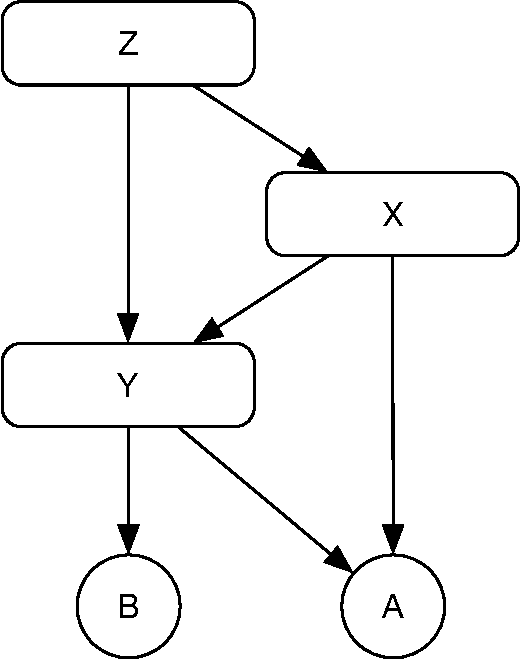
\includegraphics[width=1.5in]{dag}
\caption{A Simple Directed Acyclic Graph (DAG)}
\label{dag}
\end{wrapfigure}

As a simple example, imagine if Chain X had Chain Y as a child as well as Pattern A.  But Chain Y also had Pattern A as a child, along with Pattern B.  Both Chain X and Chain Y use Pattern A, though perhaps at different times and in different ways.  You could also imagine a Chain Z which used by Chain X and Chain Y, and thus Chain Y was also being used twice, in different ways.

Figure~\ref{dag} at right shows this very arrangement of these chains and patterns. In the computer science world, this kind of structure is known as a {\it Directed Acyclic Graph} or {\it DAG}.  It's a {\it Graph} because every object is connected to other objects with lines called {\it edges}.  It is {\it directed} because there is a clear relationship between parents and children: that is, the edges are arrows indicating who the child is.  It's {\it Acyclic} because no child can be its own ancestor: you can't have loops (or ``cycles'').  That is, all edges are pointing {\it down}.

You don't have to start playing at Chain Z.  You could instead choose to start playing at (say) Chain Y, and so Z and X would both just be ignored.  Seq calls the node that you're starting playing at the {\bf Root} of the current sequence (even if it itself has parents).

\paragraph{Seq Terminology}

Seq's sequences are DAGs built out of basic musical building blocks (step sequences, chunks of MIDI, etc.), and objects which group other building blocks into subsequences (including grouping other subsequences tother).  All these objects, both basic and grouping, are know as {\bf motifs}.  Thus (to use the LM-1's terminology) both individual step sequence patterns and pattern chains are represented as kinds of motifs.  One motif is designated the {\bf root motif}, and is the start point when playing.  Motifs which group other motifs are known as the {\bf parents} of those {\bf children}.  

When you're editing a Motif, you'll be shown the {\bf Motif Display} and, to its right, various {\bf Inspectors} to modify the features of the Motif and how it manages its children (if it has them).  All your Motifs are collected into one group, called the {\bf Motif List}.

\paragraph{Where We're Going with Seq}

Seq's sequence structure is very amenable to customization and automated modification.  Our ultimate goal is to ask what kinds of machine learning, optimization, or search techniques we could add to Seq to convert it into a {\bf co-creative tool} for the composer, that is, a tool that works with the composer, bouncing ideas back and forth, to produce a song.  We have previous experience in tools of this sort (see Sean Luke's {\bf Edisyn} for example).  But before we get to doing stuff like that, we have to get Seq finished.

\clearpage\section{The User Interface}

\begin{figure}[b]
\centering
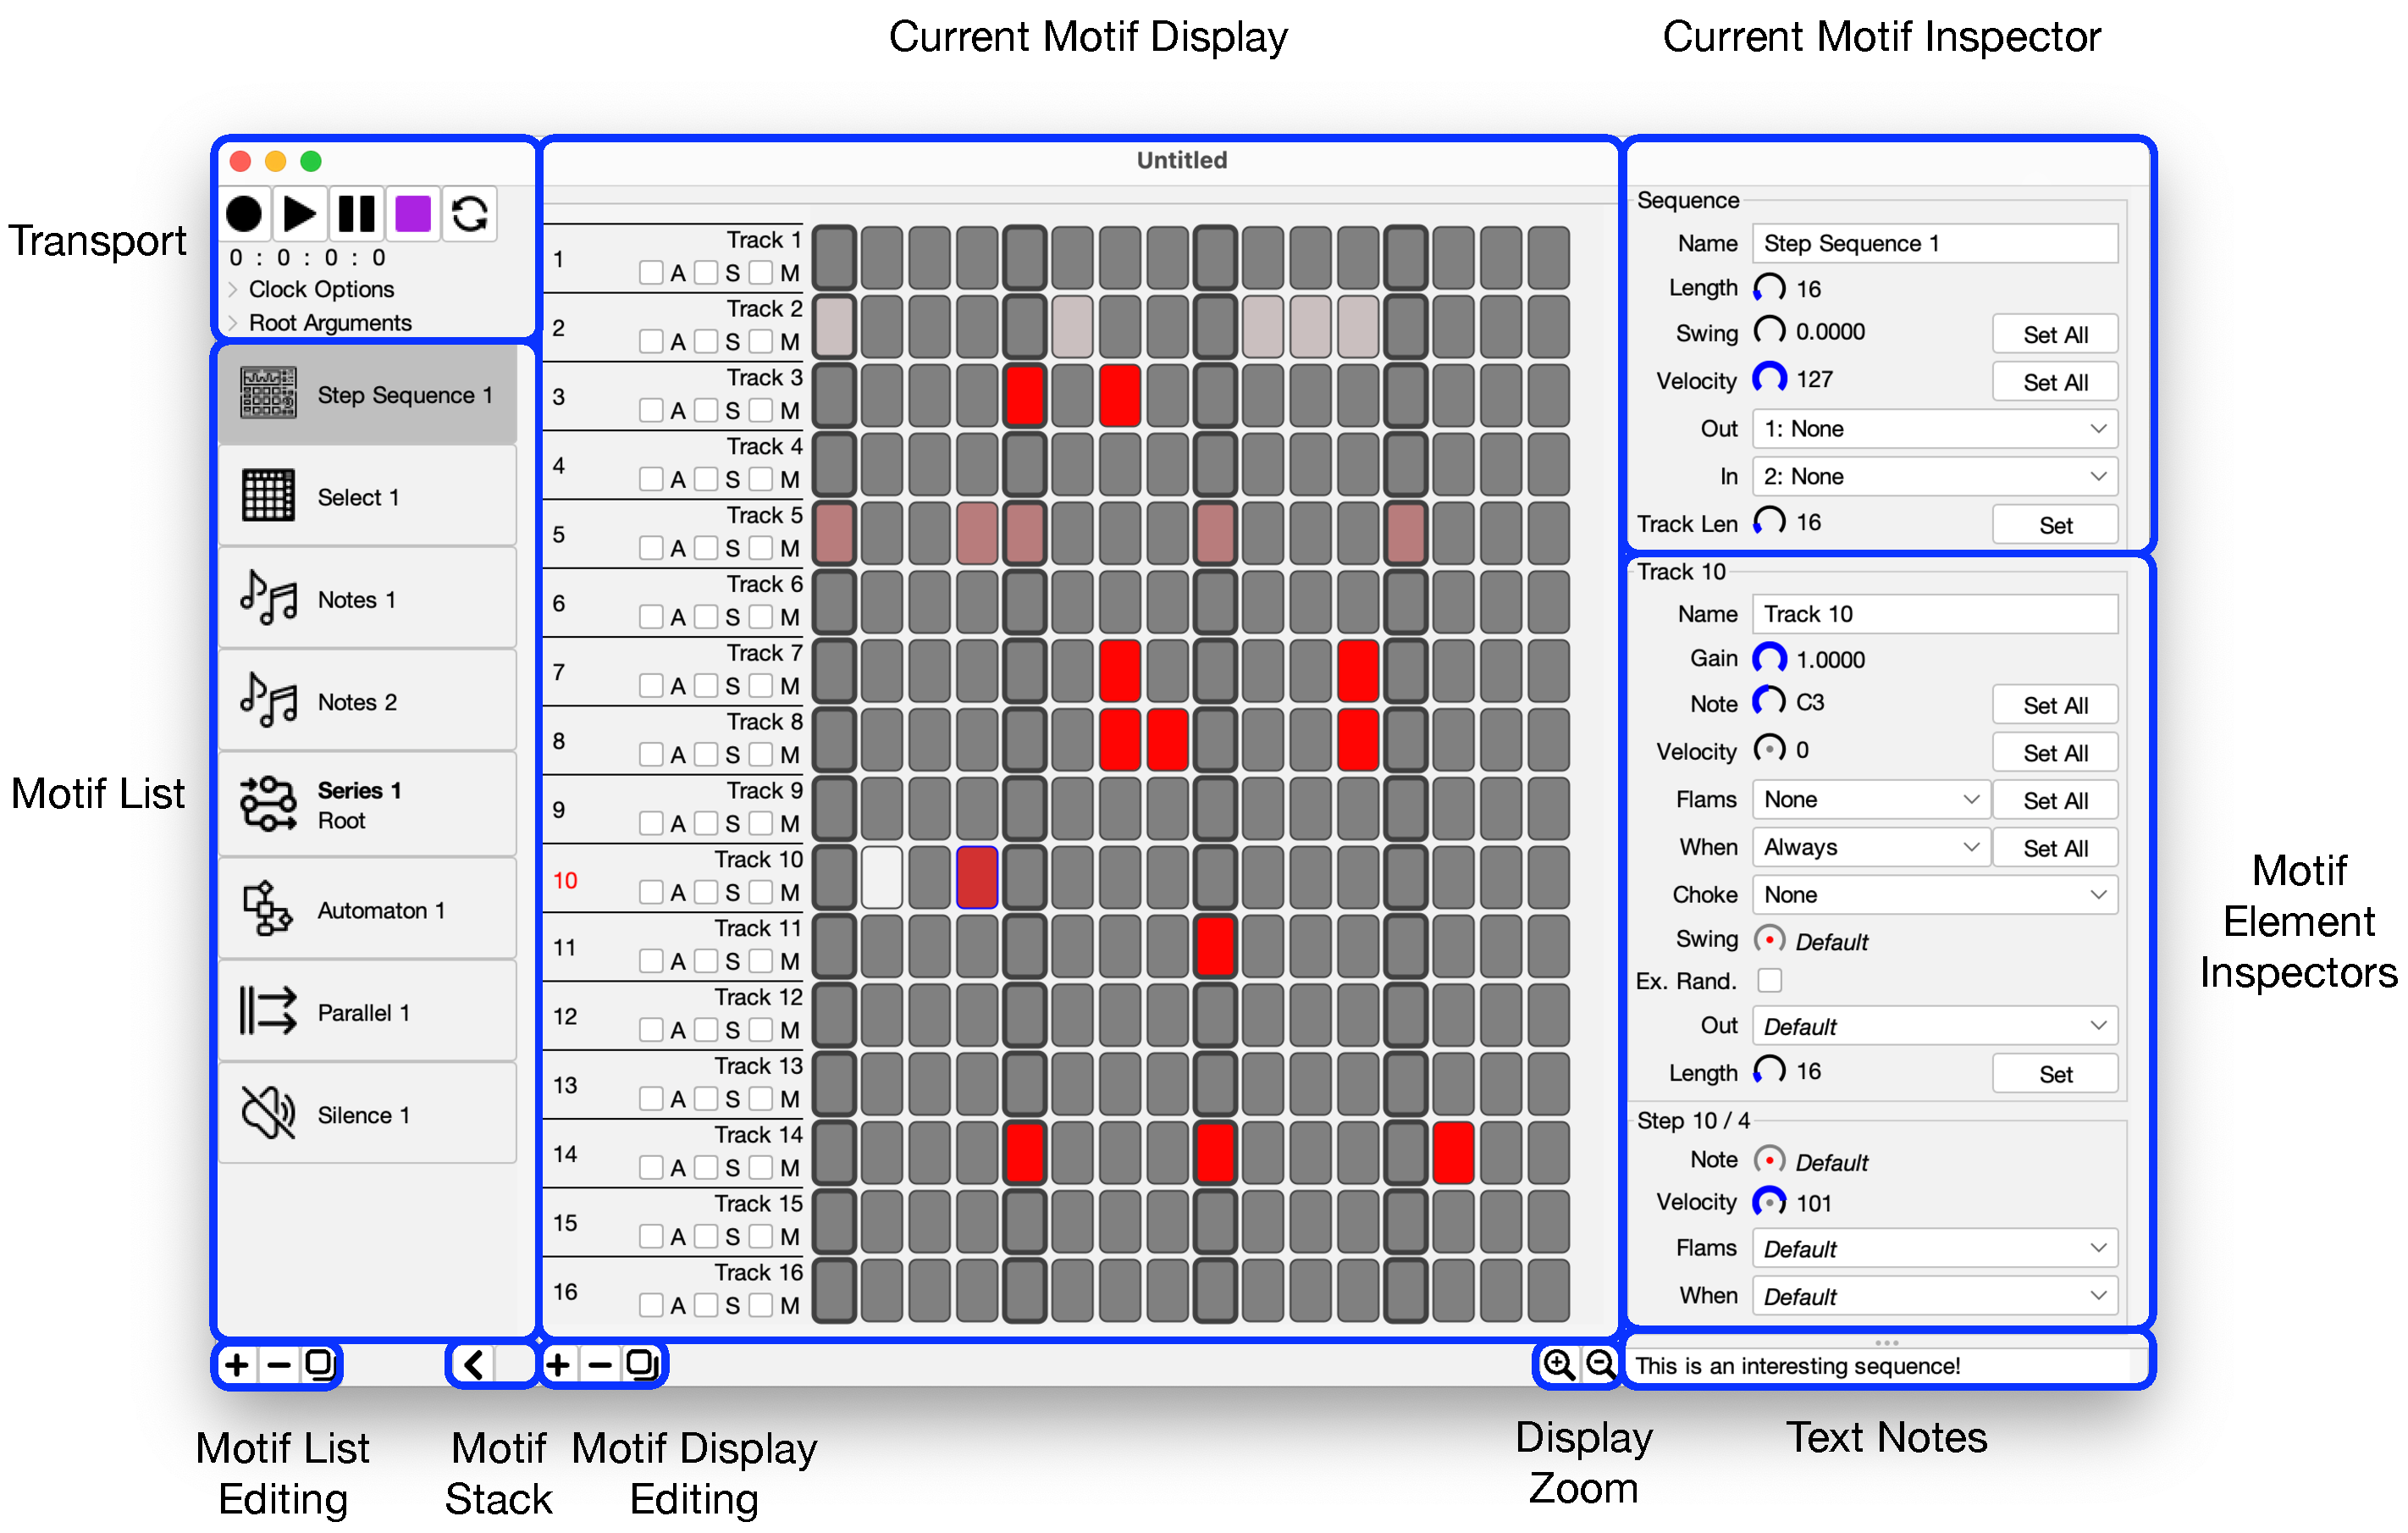
\includegraphics[width=6.5in]{MotifDisplay.pdf}
\caption{Seq graphical interface elements.}
\label{gui}
\end{figure}

Seq is organized with a single window, shown in Figure~\ref{gui}.  At top left is the {\bf Transport}, which contains the record, play, pause, stop, and loop buttons, plus the current time clock in ticks, beats, measures, and parts.  The Below the transport are two expandable regions for {\bf Clock Options} and for {\bf Root Arguments}.

Below the Transport is the {\bf Motif List}.  This is a scrollable list of every motif you have added to your sequence.  Below the Motif List are the {\bf Motif Editing Buttons} to add, remove, and duplicate motifs in the list; as well as the {\bf Motif Stack Buttons}, which let you return to previously visited motifs in order.

In the center of the window is the {\bf Current Motif Display}.  This shows the selected motif and lets you edit it.  Different motifs have different displays.  The one shown in Figure~\ref{gui} is a Step Sequence.  Below the Current Motif Display are are the {\bf Motif Display Editing Buttons}, which let you add to the display, delete from it, and copy elements in it; and the {\bf Display Zoom Buttons} which let you zoom in and out.  Different motifs have different options for these buttons.

At the right are the {\bf Inspectors}.  These are regions for editing the parameters of the current motif itself, and various elements in the motif.  At top right is the {\bf Current Motif Inspector}.  This holds editable features of the current motif.  For the Step Sequence, editor features include things such as the sequence name, length, degree of swing, etc.

Below the Current Motif Inspector are the {\bf Motif Element Inspectors}.  Different motifs have different kinds of elements, so a variety of things may appear here.  In this example, there is an inspector for the features of the currently selected Track (Track 3\,---notice this track's number is highlighted in red).  Below it is an inspector for the features of the currently selected step in this track (Step 7 of Track 3).  

Below the Inspectors is a resizable region for {\bf Text Notes} for each Motif.

\paragraph{Dials}

\begin{wrapfigure}{r}{1in}
\vspace{-1em}
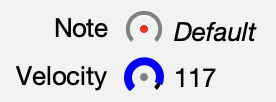
\includegraphics[width=1in]{smalldials}
\vspace{-2em}
\caption{Dials}
\label{dials}
\vspace{-1em}
\end{wrapfigure}

Most widgets are pretty standard in Seq.  But {\bf dials} require a little explanation.    A dial (usually) sets a numerical value: you set it by clicking on the dial proper and dragging up or down.  The dial then shows the numerical value to its right.   For example, the {\it Velocity} dial at right is set to 117.  

Some dials can be set to {\bf special values}.  These dials will have a little gray dot in the center of them (as was the case for the Velocity dial).  Sometimes there is only one special value.  If you double-click on the dial, it will automatically be set to this special value. If there are more than one special value, when you double-click on the dial, a menu will pop up to let you choose the special value you want.  If a special value is set, it is shown in {\it italics} and the little gray dot turns red.    For example, the {\it Note} dial  has been set to the special value {\it Default}.

If a dial has no special values available, no dot will appear.


\subsection{The Motif List\quad(and the Edit, Motif, and File Menus)}

\begin{wrapfigure}{r}{1.5in}
\vspace{-2em}
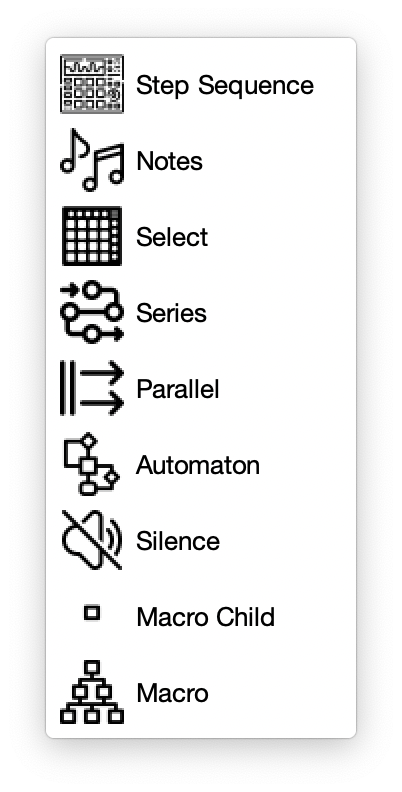
\includegraphics[width=1.5in]{motifs}
\vspace{-2em}
\caption{Available Motifs}
\label{motiflist}
\vspace{-1em}
\end{wrapfigure}

Each motif has a slot in the {\bf Motif List}, where it is shown with its current name.  You can rearrange the order of the motifs and select a new motif to display by clicking on it.  This will cause it to be displayed in the {\bf Current Motif Display}.  One motif is designated the {\bf Root Motif}, with the word {\bf Root} under the motif name.  This is the start point that will be played when the sequence is played.

When you select a motif, other motifs may appear in light blue.  These are the {\bf parents} of the motif, that is, the motifs which include the motif among their children.  Others are appear in pink: these are the {\bf children} of the motif.

When a motif is currently playing, its text will be highlighted in red.  Since a currently playing motif may also be playing its children, multiple motifs may appear in red at the same time.

Below the Motif List are the {\bf Motif List Editing Buttons}, which let you add new motifs to the list, delete them, and copy them.   Most importantly, clicking the ``\(+\)'' button will pop up the a {\bf List of Available Motifs}, as shown at right in Figure~\ref{motiflist}.  Select a motif and a new one will appear in the Motif List. 

Also below the Motif List are the {\bf Motif Stack Buttons}.  When you select a motif, the current motif display changes to reflect the newly selected motif.  The previously selected motif is pushed on the stack.  You can go back to previous motifs by pressing the ``\(<\)'' button, and return to later selected motifs with the ``\(>\)'' button.  These buttons only appear if there is a motif to go back (or forward) to.

\paragraph{Motif Menu}

The Motif Menu has several options.  

	\begin{itemize}
	\item You can {\bf set the Root Motif} to the currently selected motif.  
	\item You can {\bf automatically set} motifs to be the the Root Motif whenever you select them.  
	\item You can {\bf Sort Motifs}, which organizes motifs so that children appear lower in the list than their parents.  
	\item You can change the motif buttons to a {\bf smaller size}.
	\end{itemize}

\paragraph{File Menu}
The File Menu allows you to load and save sequences and to clear the existing sequence and restart with a new one.  You can also {\bf Export} the sequence starting at the Root Motif, discarding all motifs that are not its children nor descendants.  Finally, you can {\bf Merge} another sequence into the current one: this adds to the current sequence copies of all the Motifs in the other sequence.

\paragraph{Edit Menu}
The Edit Menu largely concerns itself with {\bf Undo} and {\bf Redo}.  However Undo works differently than you're used to: only structural changes are undone.  If you change a parameter, it's not undoable.  However you can add an undo point prior to the parameter change by choosing {\bf Checkpoint} before making the change.


\subsection{The Transport\quad (and the MIDI Menu)}

The Transport is how you play the sequence or start recording incoming MIDI.  The transport has a Record, Play, Pause, and Stop Button, as well as a Loop Toggle.  Buttons are highlighted in colors to indicate the current playing state.  Press the {\bf Play} button to start playing, and press {\bf Stop} to stop playing.  Press the {\bf Pause} button to pause or resume playing, or (if stopped) to start playing but in a paused state.  Press the {\bf Record} button to start recording.  The {\bf Loop Toggle} loops when playing: when the sequence has ended, it will start playing again.

\begin{wrapfigure}{r}{1.5in}
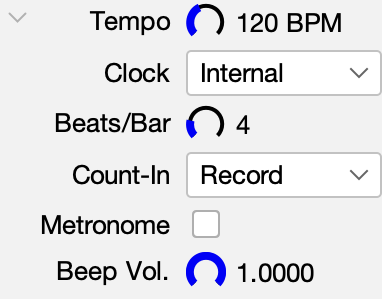
\includegraphics[width=1.5in]{clock}
\vspace{-2em}
\caption{Clock Options}
\label{clockoptions}
\end{wrapfigure}

When you start playing the sequence, play commences with the {\bf Root Motif}.  If the Root has parent motifs, they are ignored and not played.  

Recording only has an effect on certain Motifs, such as the {\bf Notes} motif, when they are armed.  Otherwise it acts just like playing for all other Motifs.

Below the Transport buttons is the {\bf Clock}, which shows the current play time in (right to left) ticks (192 ticks per beat), beats, measures, and parts (256 measures per part).  Below the clock are two expandable regions: the {\bf Clock Options} and the {\bf Root Arguments}.  The Clock Options include the tempo, whether the clock is Internal or External, the number of beats per measure, the metronome toggle, whether the metronome plays a count-in for recording, playing, or both, and the metronome volume.

We'll discuss the Root Arguments later in Section~\ref{parameters}.  However we mention one item here: the {\bf Random Seed}.  This is the seed of the random number generator used by Seq when playing, and the generator is always reset to that seed each time we play again.  That way the sequence will always be deterministic.  The seed is saved with the Sequence when you write it to a file, but new Sequences get new random seeds. You can always change this seed to cause the sequence's random choices to be different.

\paragraph{MIDI Menu}

The MIDI Menu is where you set up MIDI to play and record.  First, you with {\bf Set MIDI Devices}, you can set up to 16 {\bf Outputs} and up to four {\bf Inputs}.  Each Input or Output is a combination of a MIDI Device and a Channel.  Once you have set up an input or output. it appears as an option in device selectors for Motifs which input or output MIDI.  Inputs and Outputs are saved to preferences so you don't have to set them up each time.  You can reset from preferences by pressing the {\bf Reload} button in the setup window.

Inputs and Outputs also have {\bf Nicknames}, which are stored in preferences with them.  If you give an Input or Output a Nickname, the Nickname will appear in the selectors for various Features instead of the device name.  You'll still see the channel number.  You get rid a Nickname by deleting its text box.

You can also {\bf Panic}.  This sends an {\bf All Sounds Off} and an {\bf All Notes Off} to every setup device in order to quiet MIDI devices with stuck notes.

Finally, you can {\bf Log MIDI} to a file.  If you start this, then the next time you press Play, Seq will start copying all of its MIDI output to a MIDI file of your choosing.  The copying stops when you press Stop.  At present, if you have multiple devices, their MIDI data is merged and logged to the same file (but different channels stay separate).  

Note that some DAWs (ahem, Ableton) cannot load multichannel MIDI data -- they'll just glom it together into a single channel blob.  You probably don't want that.  Seq offers you the option of writing separate files, one for each channel.

\subsection{The Current Motif Display\quad (and the optional Per-Motif Menu)}

The current motif display varies depending on which motif you have selected in the Motif List.  Different motifs have different displays according to the nature of their data.  We'll discuss different motifs and their displays later in Section~\ref{motifs}.  

 Below the Current Motif Display are the {\bf Motif Display Editing Buttons}.  These vary depending on motifs and their need, though you might commonly see a button for adding elements, deleting them, or copying them.  For example, in Figure~\ref{gui}, the Step Sequencer display has a ``\(+\)'' for adding a Track, a ``\(-\)'' for deleting the current track, and a button for duplicating the current track.

Also below the Current Motif Display are the {\bf Display Zoom} buttons.  These zoom the display in and out and again are only appropriate for certain motifs (notably the Step Sequencer motif).

\paragraph{The Optional Per-Motif Menu}  Some motifs have their own dedicated menu which appears only when that motif is selected.  These menus will be discussed with the motifs proper in Section~\ref{motifs}.


\subsection{The Inspectors and Text Notes}

Each motif, and each element contained inside a motif, has an {\bf Inspector}.  An Inspector is a labelled list of every editable feature of the motif or element.  Inspectors appear in the column at the far right of the window.  Inspectors change a the Current Motif, or elements selected within the Current Motif, change.

At top right is the {\bf Current Motif Inspector}.  This is, unsurprisingly, the Inspector for the editable features of the Current Motif.  Different motifs will have different available features, though they will all have at least {\it one} feature: the Motif's {\bf Name}.  By default the name is something boring like ``Automaton 1'', but you can rename it to anything you want.

Some Motifs also have {\bf Parameters} their child motifs can refer to.  Each of these parameters can be custom named, and the parameter names appear as an expandable region in the Current Motif inspector.  We'll discuss parameters later in Section~\ref{parameters}.

Below the Current Motif Inspector may appear {\bf Element Inspectors}.  For example, in Figure~\ref{gui}, below the Step Sequence inspector appear Inspectors for the currently selected Track in the Sequence, and for the currently selected Step in the Track.  Many Motifs have Element Inspectors, but they vary.  Motifs that hold Child Motifs typically show an Inspector for the currently selected Child, for example.

At bottom are {\bf Text Notes}.  You can resize this region and store all the notes you like, and they will be saved with each Motif.

\clearpage\section{The Motifs}
\label{motifs}

Excluding Macros and Macro Children, there are presently seven Motifs available in Seq:

\begin{itemize}
\item Three {\bf Basic (Note-Generating) Motifs}: Step Sequence, Notes, and Silence.  These do not have children Motifs.
\item Four {\bf Compositional Motifs}: Series, Parallel, Automaton, and Select.  These have children Motifs.
\end{itemize}

We'll be adding more Motifs in time.

\vspace{1em}

Motifs are played through once, and when they have finished playing they do not themselves loop, but rather signal to their parent that they are {\bf finished}.  The parent then decides what to do with them, such as play them again, or go on to play something else, or signal to {\it its parent} that it is finished, and so on.

You can loop the entire sequence\,---\,that is, loop the {\bf Root Motif}\,---\, by toggling the Loop button in the Transport prior to or during playback.

\clearpage

\begin{figure}[t]
\centering
\includegraphics[width=6.5in]{StepSequence}
\vspace{-2em}
\caption{Step Sequence Motif.}
\label{stepsequence}
\end{figure}

\subsection{Step Sequence}

Step Sequence is one of the most complex motifs, as it is a reasonably full-featured multitrack step sequencer.  Step Sequence defines a single multitrack pattern, which is played once and then declares it is finished.  The Step Sequence can have any number of Tracks, and each Track can have any number of Steps (and that number can vary from Track to Track).  By default the Step Sequence presents itself with 16 Tracks of 16 Steps.  

\paragraph{Steps}

A Step is either {\bf off} (gray) or {\bf on}.  When on, the Step has a {\bf velocity} (volume), represented by a gradeated color between white and red.  Each Step can also have its own {\bf Note Pitch}, its own number of {\bf Flams} (ratchets), and a declaration of {\bf When} (or perhaps better called {\it whether}) the Step plays when its time is up.  The When setting can be {\it always}, or it can play with some {\it probability}, or it can play with some {\it pattern}.  An example pattern is \textsf{O O X}, which means to play the first two times the Step Sequence is iterated, and then not play the third time, and then repeat. 

All four of these features (Note, Velocity, Flams, and When) also can be set to the special value {\bf Default}.   If set this way, the feature will defer to the feature value for its Track.

Every fourth Step is bolded in the interface only for visual assistance.    The currently selected Step is outlined in blue.

\paragraph{Tracks}

A track is an iteration of Steps played one after another.  Even though tracks can have different numbers of steps, they will play their steps such that they all finish at the same time.

A Track has a {\bf Track Header} and then the list of Steps.  You can change the order of a Track in the list of Tracks by dragging its Track Header up or down.  A Track also has a {\bf Name}, which you can set in its Inspector,  Track Headers have three buttons: {\bf Arm (A), Solo (S),} and {\bf Mute (M)}.  If you select Arm, then the track is armed for recording (see {\bf Recording} below).   If you select Mute, then that track will not play.  If you select Solo, then {\it only} that track will play.

You can add, delete, and duplicate tracks with the buttons at bottom.  You can also Zoom In and Zoom Out.  The currently selected Track has its track number highlighted in red.

Tracks have a number of features in their Inspectors, beyond their {\bf Name}.

All the Steps in a given Track play their MIDI out the same MIDI Out as specified by the Track.  By default this is set to the special value {\it Default}, meaning that the Track defers to the Sequence's global setting.  A track also has a {\bf Gain} which is multiplied against the velocities of its Steps to determine their final volume.  

A track also has a default {\bf Note}, {\bf Velocity}, number of {\bf Flams} and {\bf When} for its Steps.  By default Steps defer to these values, but you can of course change them on a per-Step basis.  You can also press {\bf Set All}, which causes all Steps to reset themselves to Default for that feature.

Each track also has up to one {\bf Choke Track}: when a Step in the Track is played, any playing sound in the Choke Track is immediately stopped (a MIDI Note Off is issued).  Tracks also have some degree of {\bf Swing} (syncopation).  A typical amount of swing would be about 30\% (if you wanted Swing), else 0\%.

A Track can be a member of the {\bf Exclusive Random Group} (or ``Ex. Rand.'').  When the Sequence is played, one and only one Track in the Exclusive Random Group is played; the others are hushed (independent of Mute settings).  The Track in question is selected at random. Tracks not in this group are not effected.

Finally, a track has a {\bf Length}, that is, the number of steps.  This is not set until the {\bf Set} button is pressed.

\paragraph{The Step Sequence Inspector}

At top, the Step Sequence inspector defines the global settings for the Step Sequence.  There is its {\bf Name} of course.  After this there is the {\bf Duration}, that is, the length of time (in 16th notes) that this Step Sequence will take to complete.  For example, even if the Step Sequence is 16 steps long, if you set the Duration to 4, it'll run at the speed necessary to complete those 16 steps in one quarter note of time.  The default is of course 16: 16 steps in 4 quarter notes.

You can also set the default {\bf Swing}, {\bf Velocity}, and {\bf Out}, and Tracks will defer to these if set to {\it Default}.  The {\bf Track Length} indicates the initial number of Steps for newly added Tracks. Finally, {\bf In} specifies the MIDI Input to use when recording tracks.

\paragraph{Recording a Step Sequence}

If you arm one or more Tracks, set their Notes, and set the Sequence's MIDI Input accordingly, then you can record in Notes to those tracks when you press Record on Seq.   You will find this easier if you turn on the metronome and if you set the Step Sequence to be the Root, so it records immediately.  Remember that if your Step Sequence motif is not a descendant of the Root, it will never be reached to do Recording.



\clearpage

\begin{figure}[t]
\centering
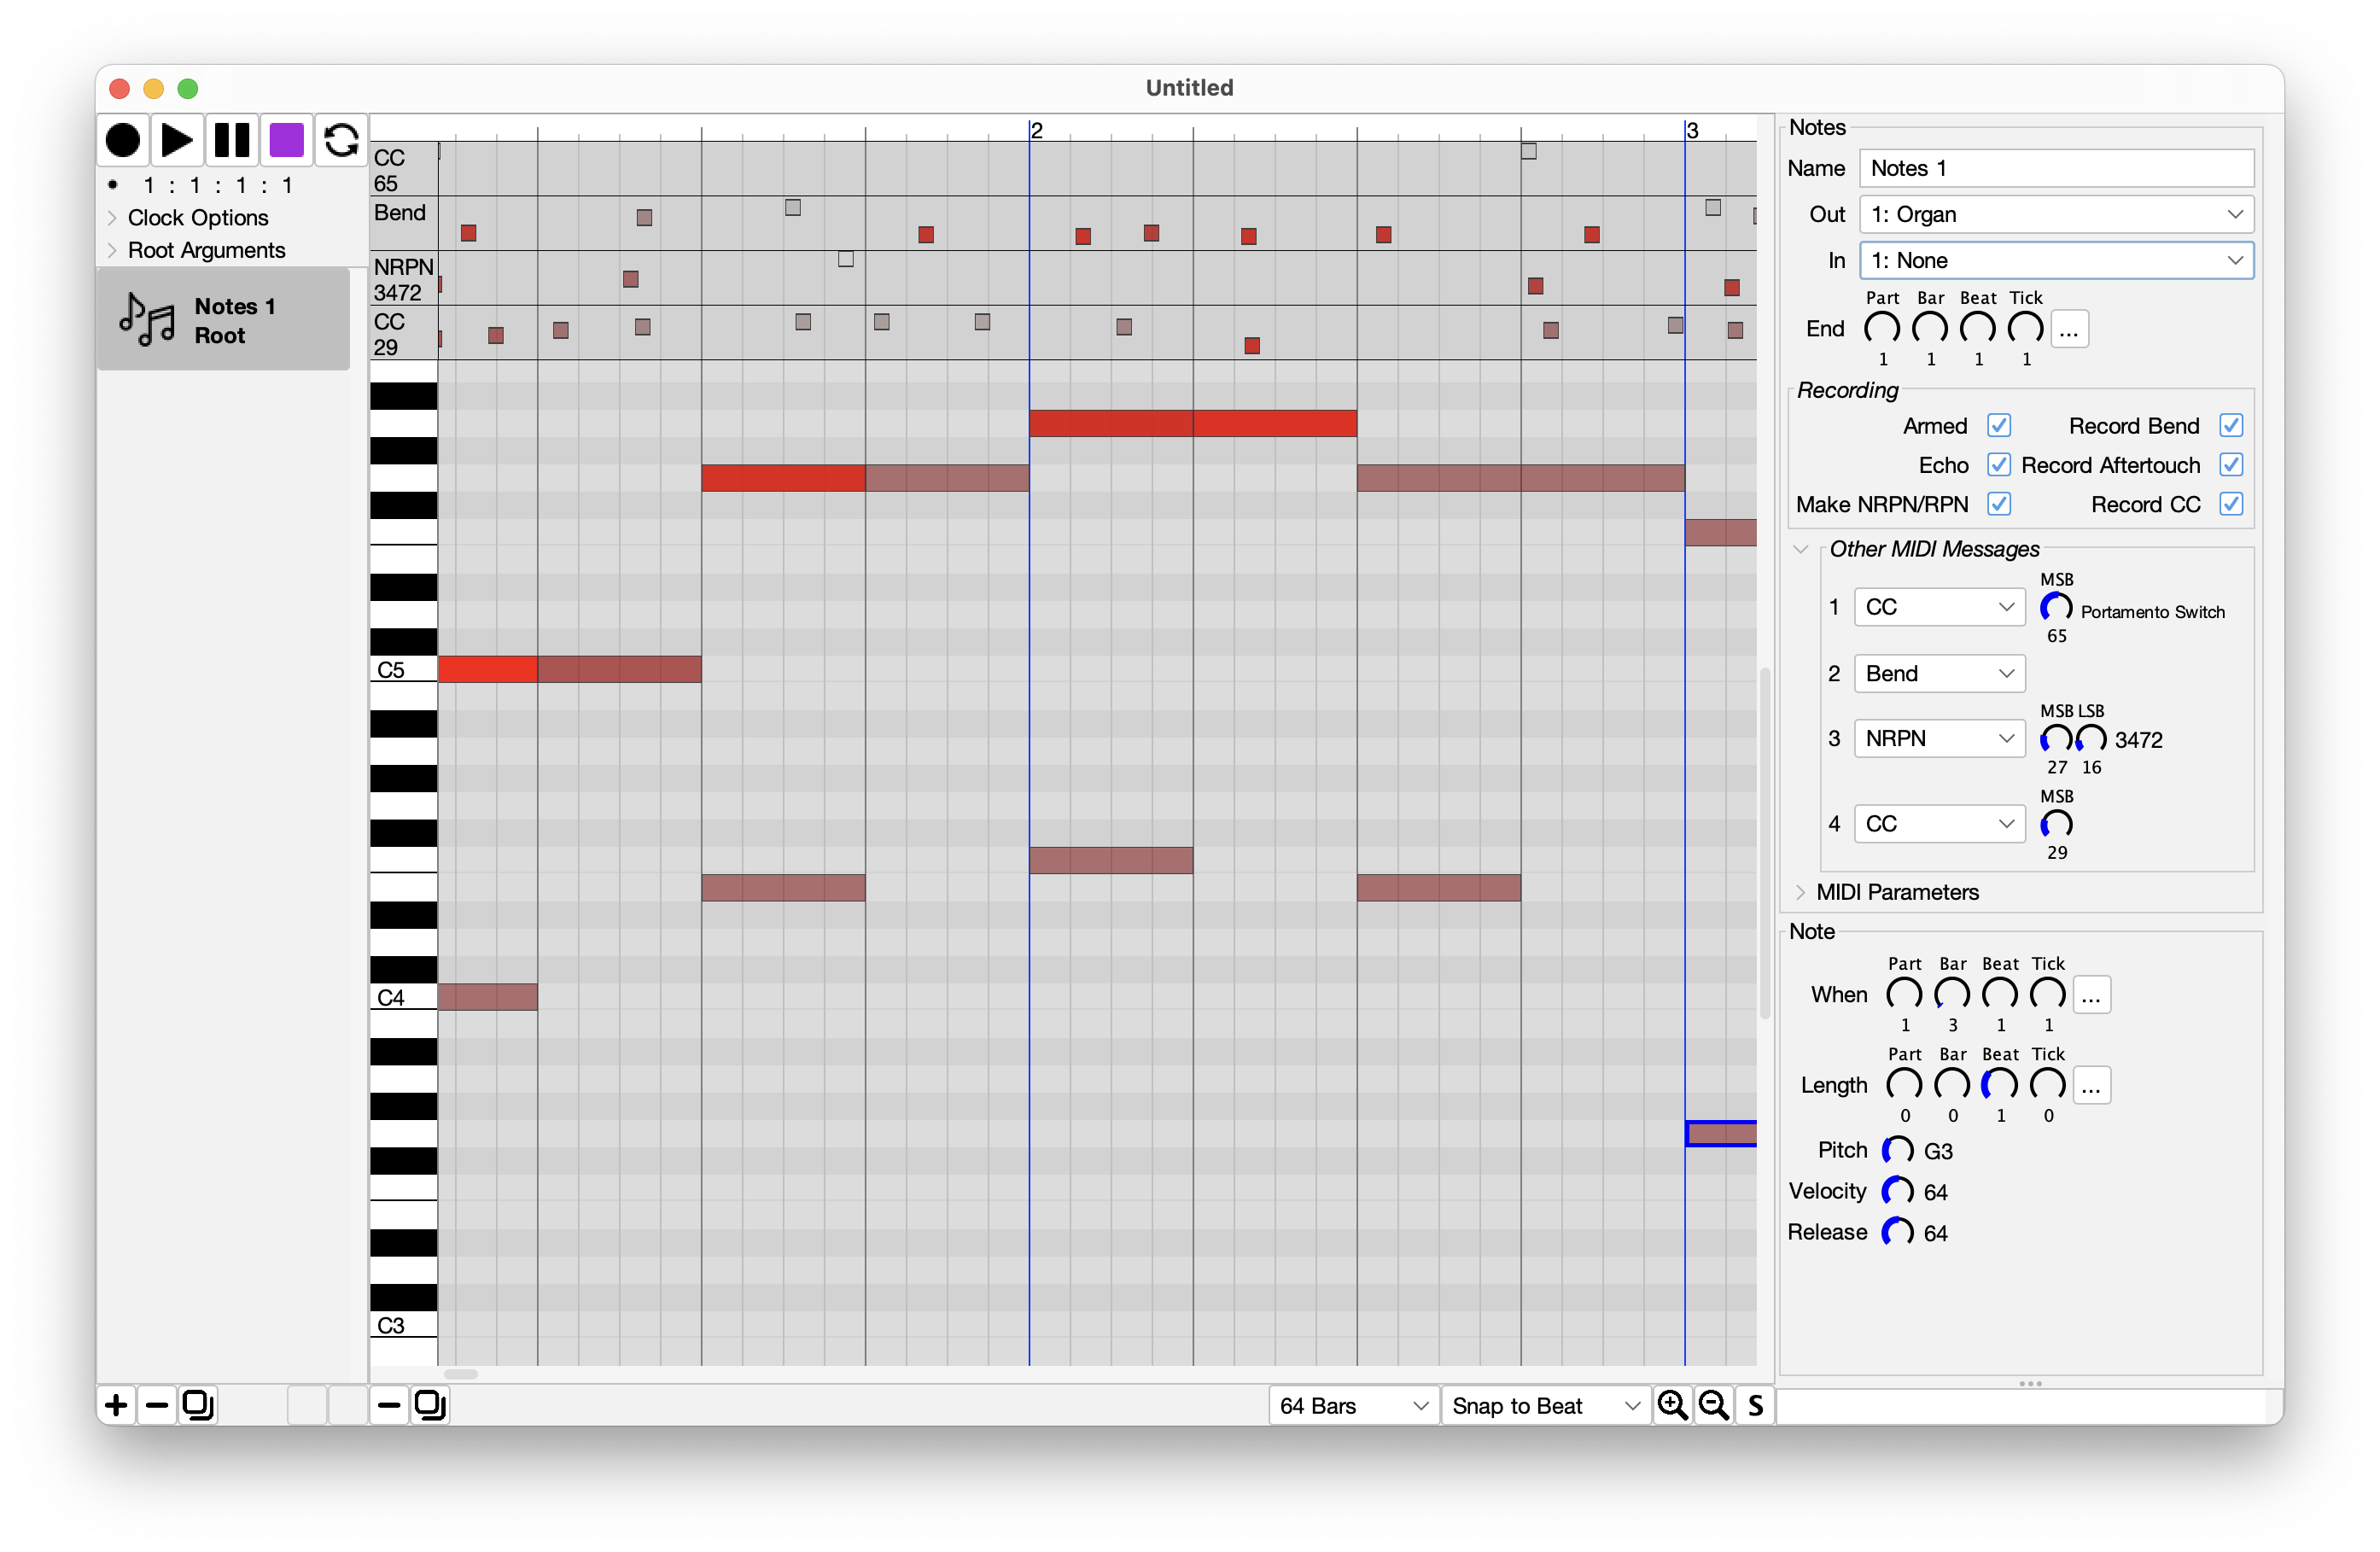
\includegraphics[width=6.5in]{Notes}
\vspace{-2em}
\caption{Notes Motif.}
\label{notes}
\end{figure}

\subsection{Notes}
 
Notes is simply a collection of MIDI events: MIDI Notes, Pitch Bend events, CC events, and Aftertouch Events.  Notes are not stored as MIDI Note On/Note Off, but as entire notes with an onset, pitch, velocity, length, and release velocity.   When Notes is played, it plays through all its events in order once.

\paragraph{\color{red} To Do} We still haven't built a proper Note Editor for Notes.  At present it's still just displaying its Notes as a table.  It's a big job but one that is frankly low priority.  For now you'll need to edit your Notes by exporting them to a MIDI file, loading them in your DAW, editing them, and then re-importing them.

Notes has a MIDI Out and a MIDI In.  The MIDI Out is of course where the MIDI events go.  The MIDI In is the source of events when recording into Notes.

You can select ranges of notes (for various menu actions), and when Notes is playing, it will highlight the last event played (and scroll to it).

\paragraph{Notes and Events} The Notes object supports four kinds of events: Notes, Pitch Bend, CC, and Aftertouch.  If you select an event, its inspector pops up.  All four events have a time of onset called {\bf When}.  You can change this value, but you must press {\bf Set} to set it, because it will change the order of the note in the list.

Notes also have a {\bf Length}, a {\bf Pitch}, a {\bf Velocity} (volume), and a {\bf Release Velocity}.  Note that the velocity cannot be set to 0.  The Length comes with some useful presets.  Unlike When, changing Length is immediate.

Pitch Bend has a bend value called, not surprisingly, {\bf Bend}. It's positive or negative.

CC events each have a {\bf Parameter} and a {\bf Value}.

Aftertouch events each have a {\bf Pitch} and a {\bf Value}.

\paragraph{Recording Notes} To record notes, first make sure that its {\bf MIDI In} is set to your device.  Then {\bf Arm} the Notes in its Inspector, press Record in Seq, and record in some notes.  You'll find it easier if you turned on the Metronome.  If you select {\bf Echo} in the Inspector, then all events received via the MIDI In will be echoed out the MIDI Out: you probably would want that.  Remember that if your Notes motif is not a descendant of the Root, it will never be reached to do Recording.

\paragraph{The Notes Menu} Notes has a number of items under its menu:

\begin{itemize}

\item{\bf Load MIDI File...}\quad will load MIDI data from a MIDI file, replacing the existing data.

\item{\bf Quantize...}\quad gives options for quantizing all or a range of your notes or event data. 

 A note about  the {\bf quantization bias}.  What is this?  Normally quantizers just round the notes up or down to the nearest quantized position, but this is often wrong.  As a human, you may tend to play more notes early than late (or vice versa), resulting in an error distribution which is {\it ought} to favor the earlier quantized positions more than the later one (or vice versa).  You can set the bias to match your personal tendencies.

\item{\bf Shift Time...}\quad gives options for stretching a region of notes to fill a different amount of time.

\item{\bf Stretch Time...}\quad stretches the time of the selection, or the whole  the time of the onset of all or a range of your event data by a given amount.

\item{\bf Trim Blank Time from Start}\quad deletes empty time from the start of your data.  Your first event will start at timestep 0 in the Notes.
\item{\bf Delete Selection}\quad deletes the selected events.

\item{\bf Randomize Time...}\quad gives options for adding noise to the onset and optionally the duration all or a range of your notes or event data.

\item{\bf Transpose...}\quad transposes the pitch all or a range of your notes by a given amount.

\item{\bf Set Velocity...}\quad lets you set the velocity of all notes in a range or all notes in the motif.

\item{\bf Randomize Velocity...}\quad gives options for adding noise to the velocity of all or a range of your notes.

\item{\bf Delete Selection}\quad deletes the selection.

\item{\bf Filter...}\quad gives options for filtering out (deleting) notes, bend data, CC data, or aftertouch data.

\item{\bf Add Note}\quad adds a note and selects it.

\end{itemize}


\clearpage

\begin{figure}[t]
\centering
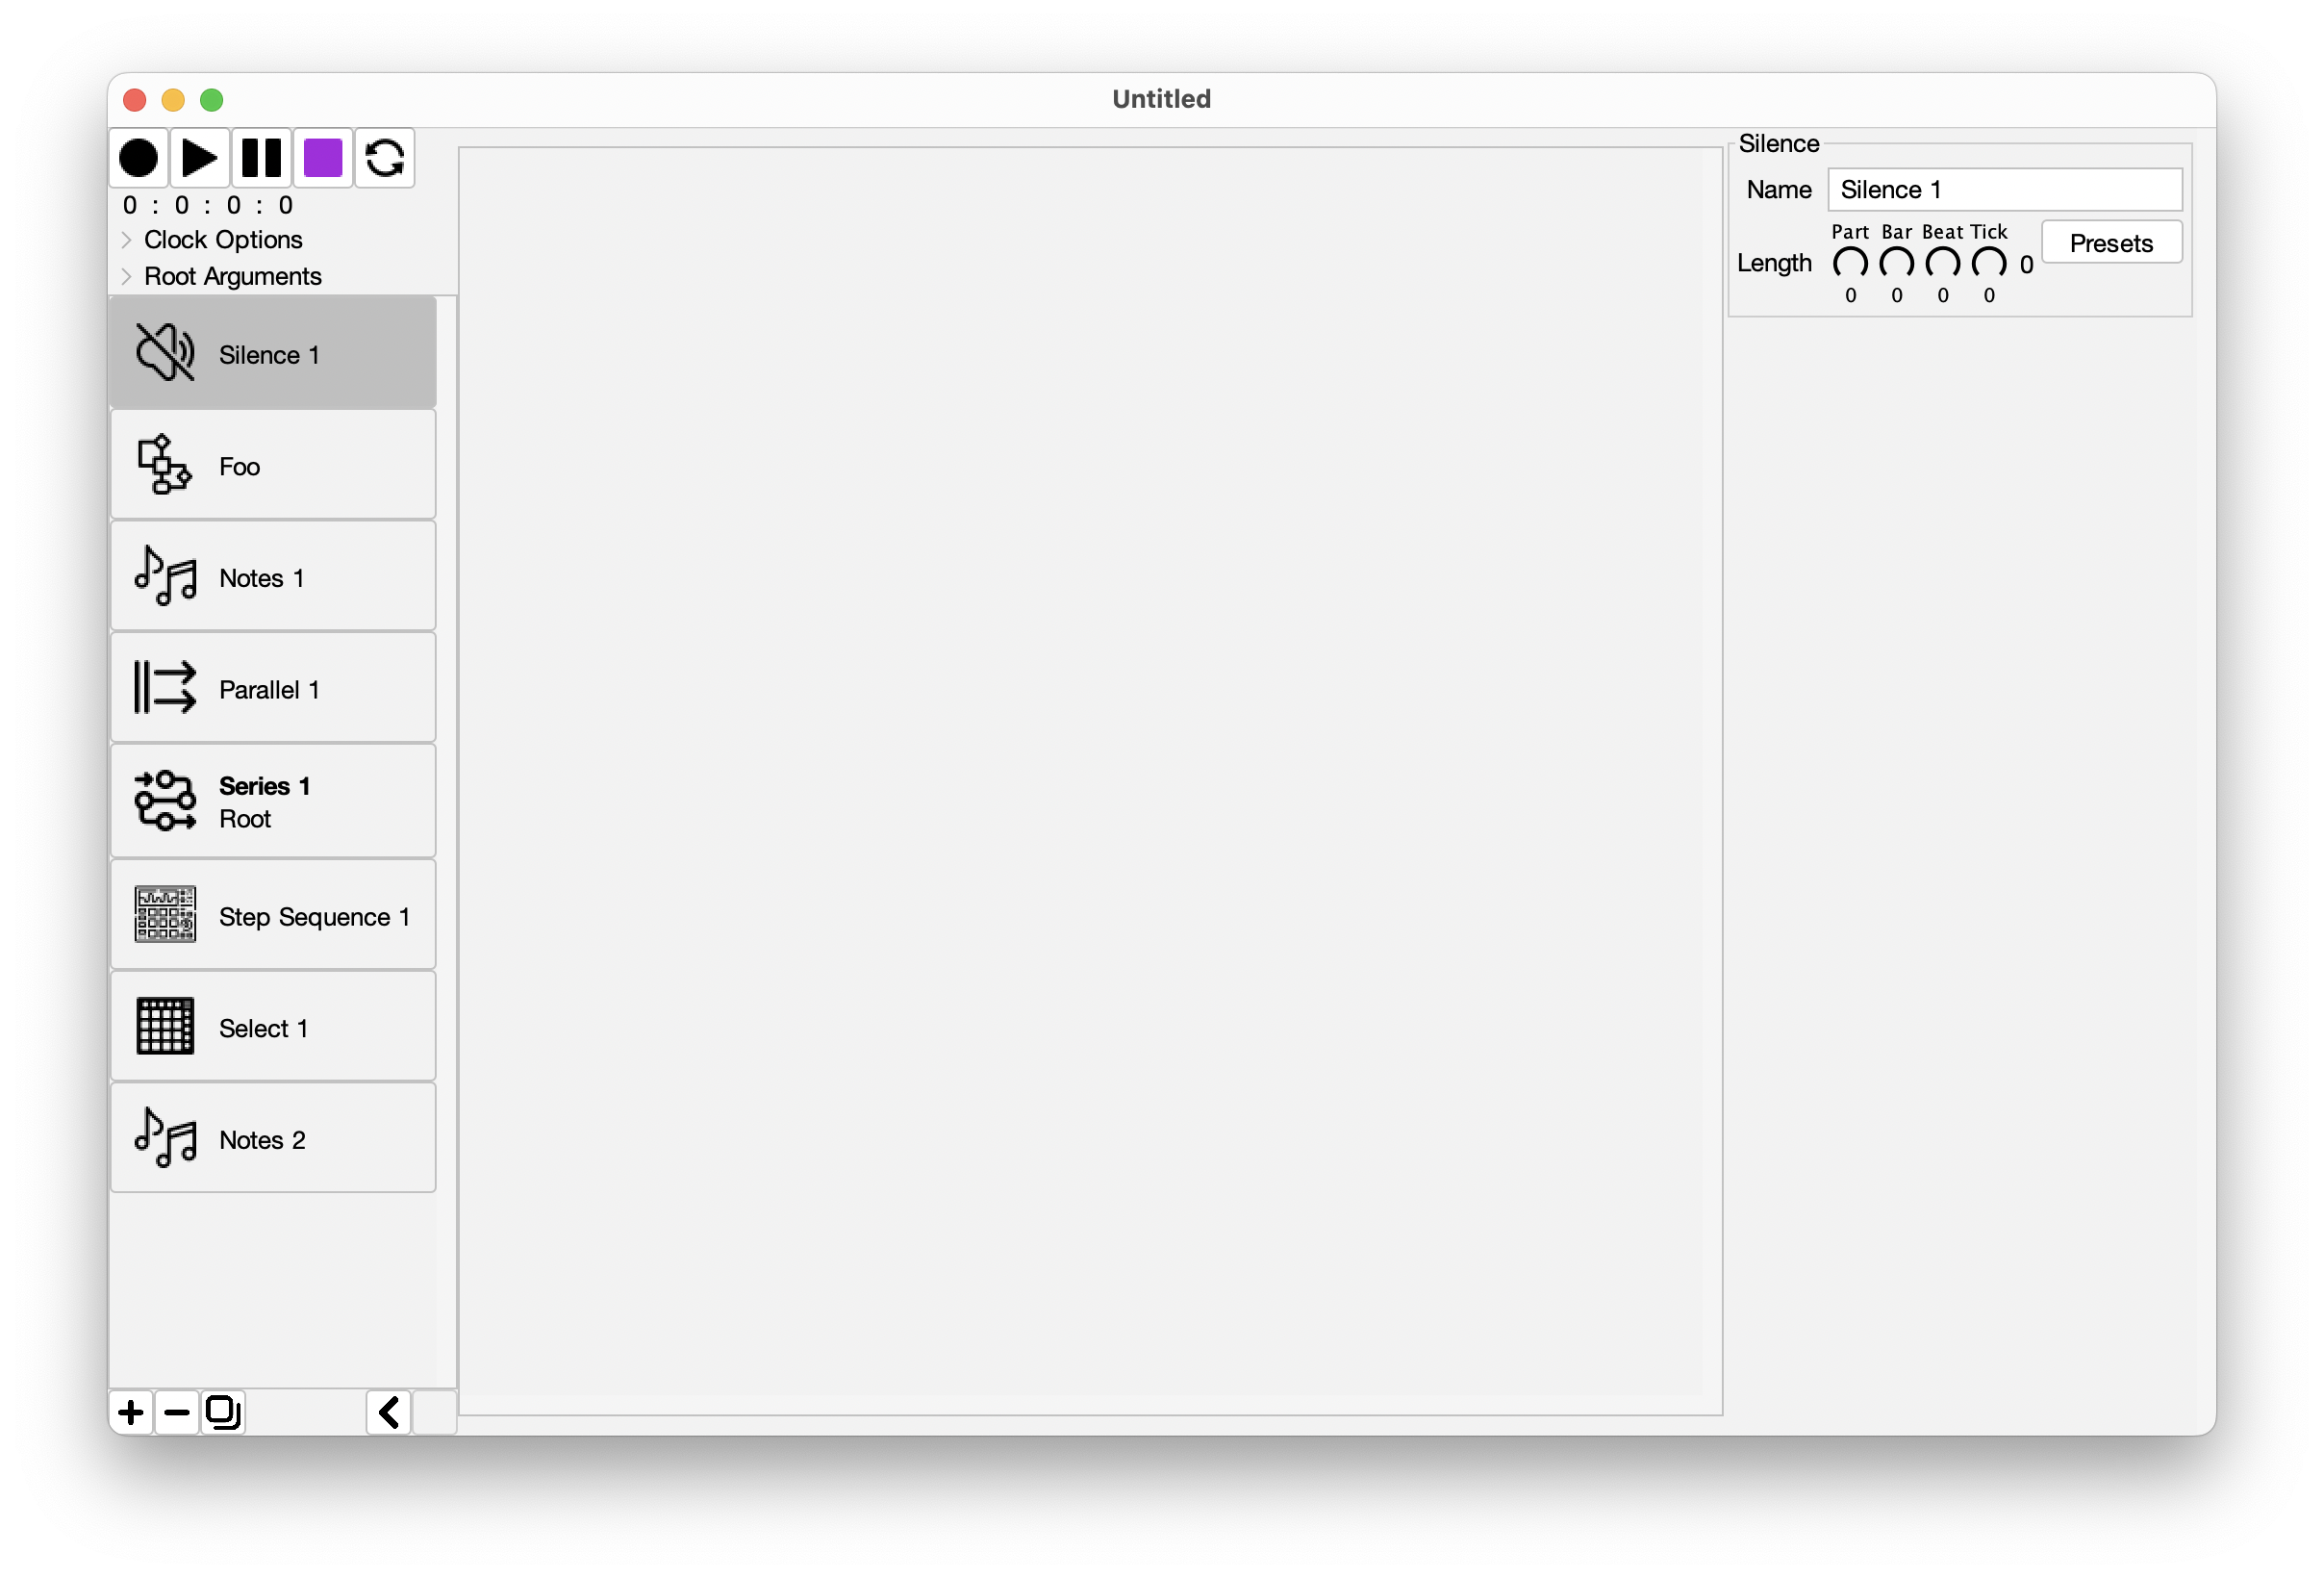
\includegraphics[width=6.5in]{Silence}
\vspace{-2em}
\caption{Silence Motif.}
\label{silence}
\end{figure}

\subsection{Silence}

Silence is nothing more than a fixed-length chunk of silence.    You can specify the {\bf length} in parts, bars (measures), beats, and ticks.  There are 192 ticks per beat, and 256 bars per part.  The number of beats per bar depends on your clock settings.  As this is tedious, you can also select from some {\bf presets}.


\begin{figure}[t]
\centering
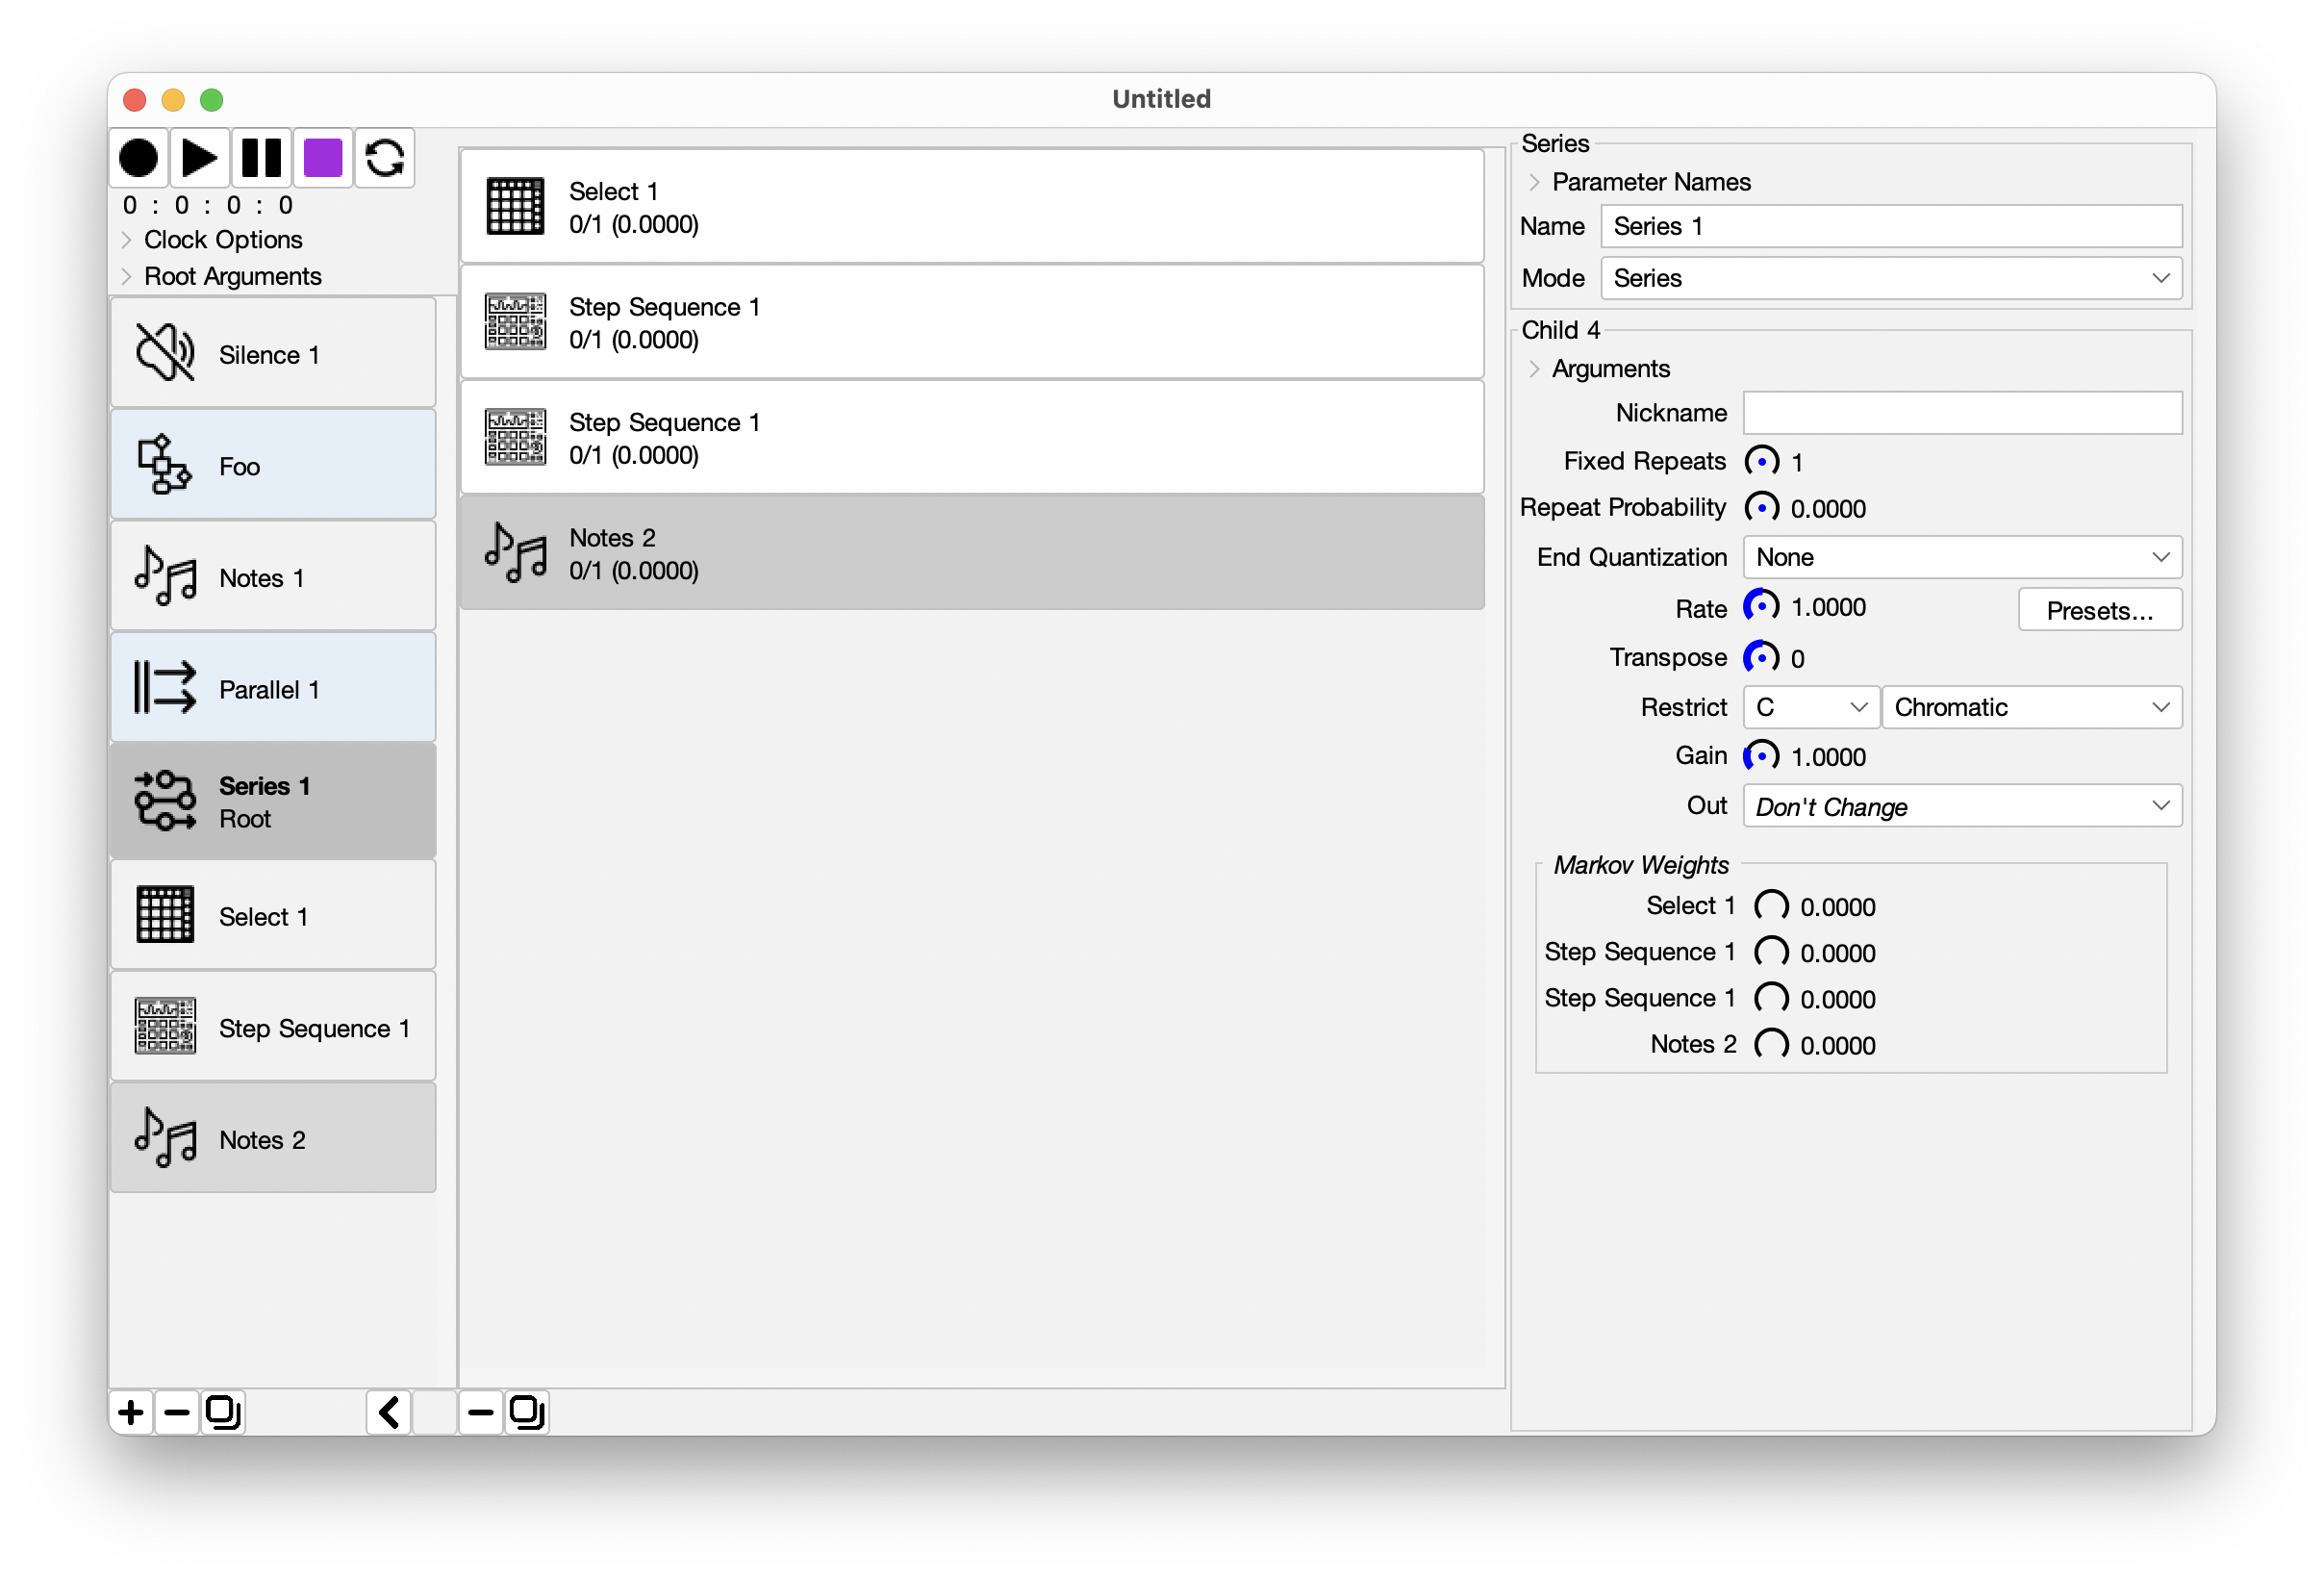
\includegraphics[width=6.5in]{Series}
\vspace{-2em}
\caption{Series Motif.}
\label{series}
\end{figure}

\clearpage\subsection{Series}

By default Series is exactly what it suggests: a series of child motifs played one after another.   By ``Play'' we mean that a Child Motif is played until it is finished, and then this is repeated some \(N\) times.  That is, Series is essentially Song Mode.  

But in fact Series has several modes, and so can be set to play its children in a number of ways:

\begin{itemize}
\item{\bf Series}\quad Play each child in sequence, then finish.
\item{\bf Shuffle}\quad Randomly shuffle the order of the children.  Then play them in that order, then finish.
\item{\bf Random Forever}\quad Select a random child to play.  When finished playing it, select another one at random and play it, and so on.  Do this forever.  
\item{\bf Random Markov}\quad Select a random child to play.  When finished playing it, select a second one at random using the first child's Markov Weights, and play it.  Then select a third child at random using the second child's Markov Weights, and so on.  Do this forever.
\item{\bf Variation}\quad Play the child specified by Parameter 1, then finish. (For discussion of Parameters, see Section~\ref{parameters}).  This is particularly useful for creating and playing multiple {\it variations} of a given Motif.
\item{\bf Random Variation}\quad Play the child specified by the Random Parameter, then finish. (For discussion of Parameters, see Section~\ref{parameters}).
\end{itemize}

The {\bf Mode} is specified in the Series Inspector.

\paragraph{Children}

In the Current Motif Display, Series maintains a list of Child Motifs that it plays in some order or otherwise selects from.  You can drag Motifs into this list directly from the Motif List.  You can drag the same Motif to appear multiple times in the Child list.  You can also rearrange the Motifs in this list by dragging them, and can delete or duplicate a Motif in the list.

While a Child is playing, its name is highlighted in red in the Child List.

\paragraph{Child Features}
Each Child in the Child Motifs can have a {\bf Nickname}, set in its Child Inspector.  Even if a Motif appears multiple times in the List, each entry can have a different Nickname.  When you set the Nickname, it appears with the Child in the list.

When a Child finishes playing once, we can immediately go on to whatever is next to do, or we can first wait until some quantized time boundary (16th note, quarter note, or measure) before doing so.  This is set in the Inspector as {\bf End Quantization}.

When a Child is played, it is played for some number of iterations or {\bf Fixed Repeats}.  You can set this value in the Inspector.  Thereafter, we flip a coin of {\bf Repeat Probability}, and each time it comes up heads, we play the Child once more. When it comes up tails, we stop playing the child, and go on to the next step (starting playing some other child, or finishing).  These two values are also displayed in the Child in the list, along with the number of iterations performed so far.

Alternatively if you select {\bf Until Trigger 8}, both Repeats features are ignored and the Child  will repeat forever until the Series receives a Trigger on Parameter 8.  (For discussion of Parameters, see Section~\ref{parameters}).

One Child is designated the {\bf Start}.  You choose it by selecting ``Start Here''.  If you are in {\it Series Mode}, and the Series is the {\it Root}, then when you press play, playing will begin with that Child.  If no Child is designated the Start, then the Start is 0.  The purpose of this mechanism is to temporarily allow you to change where in the song you'd like to start playing or recording.

\paragraph{MIDI Modification}

As a Child of the Series emits MIDI, that MIDI is handed to the Series, which has a chance to modify it before it is passed on.  There are several available features for modification of a given Child's MIDI in its Inspector.  {\bf Transpose} transposes all notes by some number of semitones up or down.  {\bf Restrict} forces the notes to line up with notes in a given scale: notes that don't match are transposed down to the nearest note in the scale.  {\bf Gain} changes the overall volume (velocity) of notes.  And {\bf Out} changes the MIDI Out being used (by default it is set to {\it Don't Change}.

Finally, {\bf Rate} changes the speed at which the child is played, faster or slower.  Keep in mind that Seq has a resolution of 192 ticks per beat (PPQ), so changing the speed\,---\,particularly faster\,---\,can quickly result in inaccuracies.  Some {\bf Presets} are provided, including a Custom Rate option)

\paragraph{Markov Weights}

If the Series's mode is Random Markov, the first child to play is selected entirely at random, but each subsequent child is selected using the Markov Weights of the current child.  The Markov Weights of a child are part of its features.  For a given child, each subsequent child is assigned a weight from 0.0 to 1.0 indicating the probability that it will be selected next time.  The weights are normalized to form probabilities.

For example, if you have three children, A, B, and C, and you have set A's Markov Weights to be A: 0.5, B 0.5, C 0.0, then after A has finished playing, either A or B will be selected next with equal likelihood.

\paragraph{Parameters and Arguments}

The Series Inspector has an expandable region called {\bf Parameter Names}, and each Child Inspector has an expandable region called {\bf Arguments}. Furthermore, many dials have Special Values called ``Rand'', ``Param 1'', etc.  These are explained in Section~\ref{parameters}.

\clearpage

\begin{figure}[t]
\centering
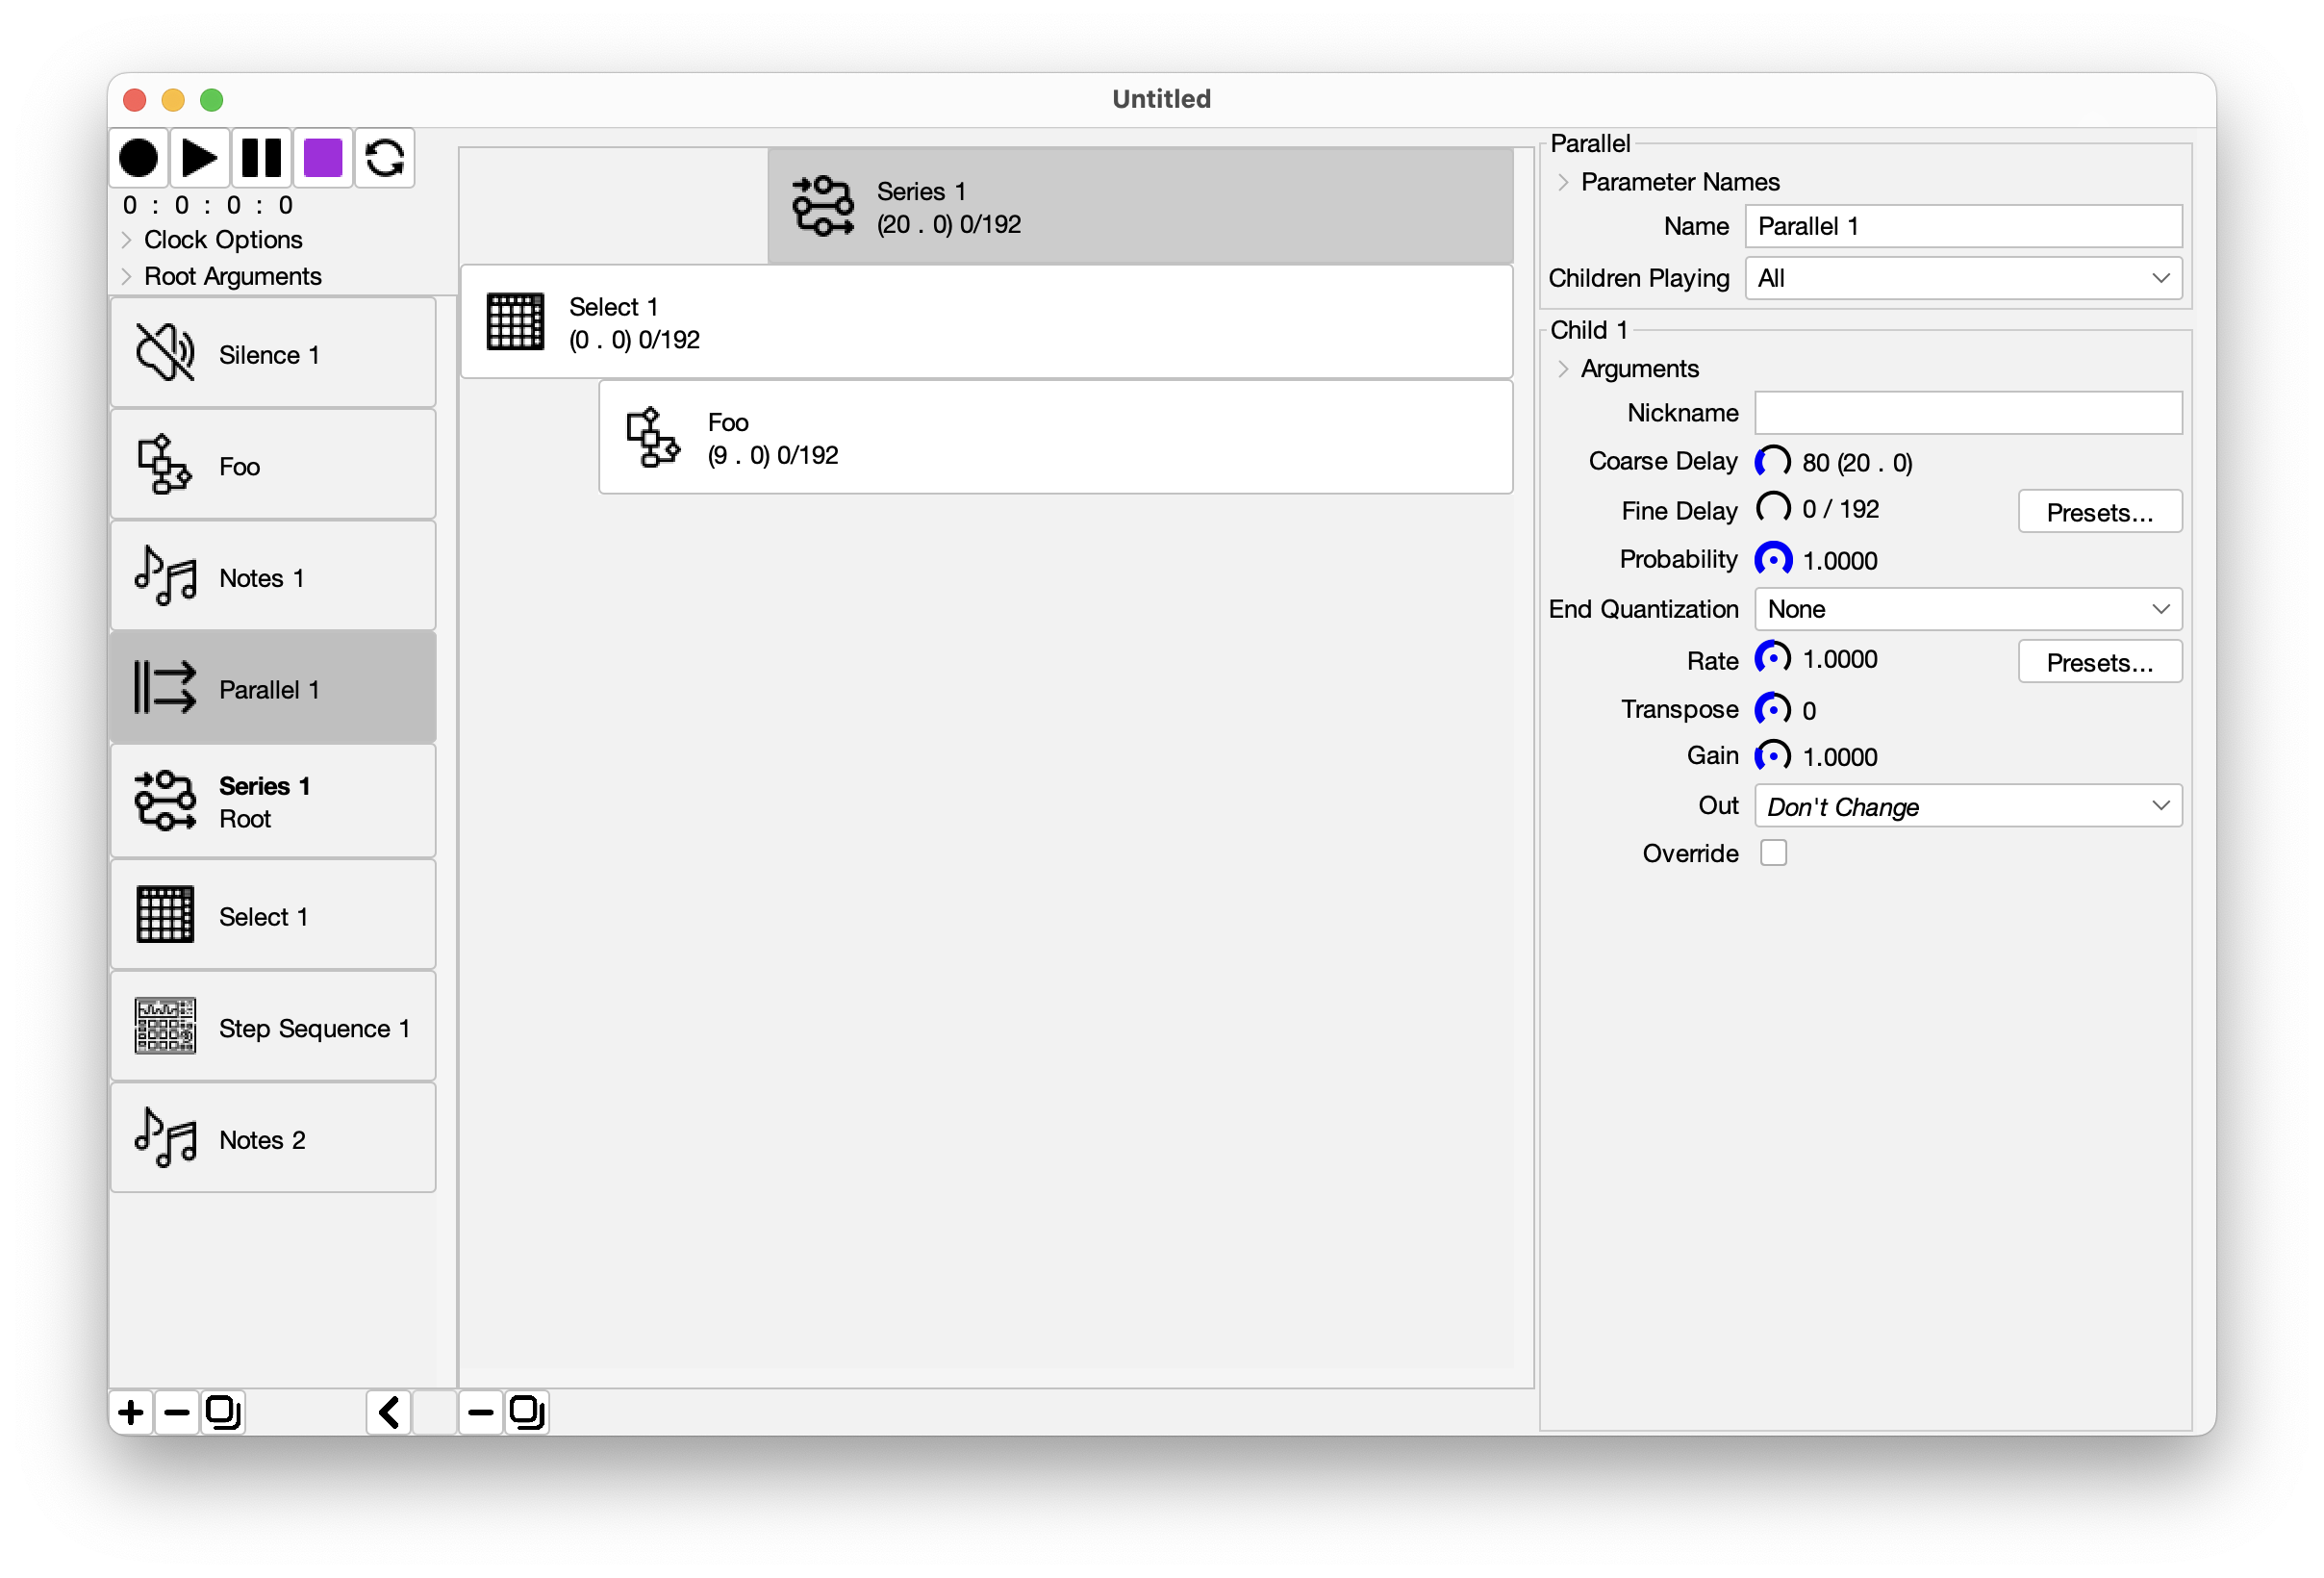
\includegraphics[width=6.5in]{Parallel}
\vspace{-2em}
\caption{Parallel Motif.}
\label{parallel}
\end{figure}

\subsection{Parallel}

Like Series, Parallel is a list of of Children; but it plays them in parallel.  Each child can have its onset delayed, so that they start at different times.  And Children can have some probability as to whether they're played at all.

\paragraph{Children}

In the Current Motif Display, Parallel maintains a list of Child Motifs that it plays in some order or otherwise selects from.  You can drag Motifs into this list directly from the Motif List.  You can drag the same Motif to appear multiple times in the Child list.  You can also rearrange the Motifs in this list by dragging them, and can delete or duplicate a Motif in the list.

While a Child is playing, its name is highlighted in red in the Child List.

Each Child in the Child Motifs can have a {\bf Nickname}, set in its Child Inspector.  Even if a Motif appears multiple times in the List, each entry can have a different Nickname.  When you set the Nickname, it appears with the Child in the list.

\paragraph{Play Probability}

Each Child has a {\bf Probability} in its Inspector.  This probability determines whether the child will be played as follows.  In the Parallel Inspector there is a feature called {\bf Children Playing}.  This feature allows you to select some \(N\) children to play when the Parallel starts playing.  Its options are:

\begin{itemize}
\item {\bf Independent}\quad Each child will play with its given Probability.
\item {\bf 1...16}\quad Parallel will select some \(N\) (1...16) children at random given their Probabilities.  These will be the only children that play.
\item {\bf All}\quad Every child will play.  This is the default.
\item {\bf All, Finish After First}\quad Every child will play, but after the first child in the list has finished playing, all children will immediately be terminated.
\end{itemize}

If a child has {\bf Override} set in its Inspector, then when it starts playing, it will immediately terminate all Children below it.  

\paragraph{Delays and Quantization}

Each Child can have the onset of its playing delayed.  Seq provides a {\bf Coarse Delay} in Beats and Measures, and a {\bf Fine Delay} in Ticks (192 Ticks per Beat).  The Fine Delay also has {\bf Presets} with common fractions of a Beat.

When the last Child finishes playing once, we can finish Parallel immediately, or we can first wait until some quantized time boundary (16th note, quarter note, or measure) before doing so.  This is set in its Inspector as {\bf End Quantization}.

When a Child is delayed, it will shift horizontally to demonstrate this, as is shown in Figure~\ref{parallel}.


\paragraph{MIDI Modification}

As a Child of the Parallel emits MIDI, that MIDI is handed to the Parallel, which has a chance to modify it before it is passed on.  There are several available features for modification of a given Child's MIDI in its Inspector.  {\bf Transpose} transposes all notes by some number of semitones up or down.  {\bf Restrict} forces the notes to line up with notes in a given scale: notes that don't match are transposed down to the nearest note in the scale.  {\bf Gain} changes the overall volume (velocity) of notes.  And {\bf Out} changes the MIDI Out being used (by default it is set to {\it Don't Change}.

Finally, {\bf Rate} changes the speed at which the child is played, faster or slower.  Keep in mind that Seq has a resolution of 192 ticks per beat (PPQ), so changing the speed\,---\,particularly faster\,---\,can quickly result in inaccuracies.    Some {\bf Presets} are provided, including a Custom Rate option)

Unlike in other Motifs, you can {\bf Mute} children in a Parallel.  The children will still have the same length and override: they just won't produce any notes.  They will produce CC and similar data (for now).

\paragraph{Parameters and Arguments}

The Parallel Inspector has an expandable region called {\bf Parameter Names}, and each Child Inspector has an expandable region called {\bf Arguments}. Furthermore, many dials have Special Values called ``Rand'', ``Param 1'', etc.  These are explained in Section~\ref{parameters}.


\clearpage

\begin{figure}[t]
\centering
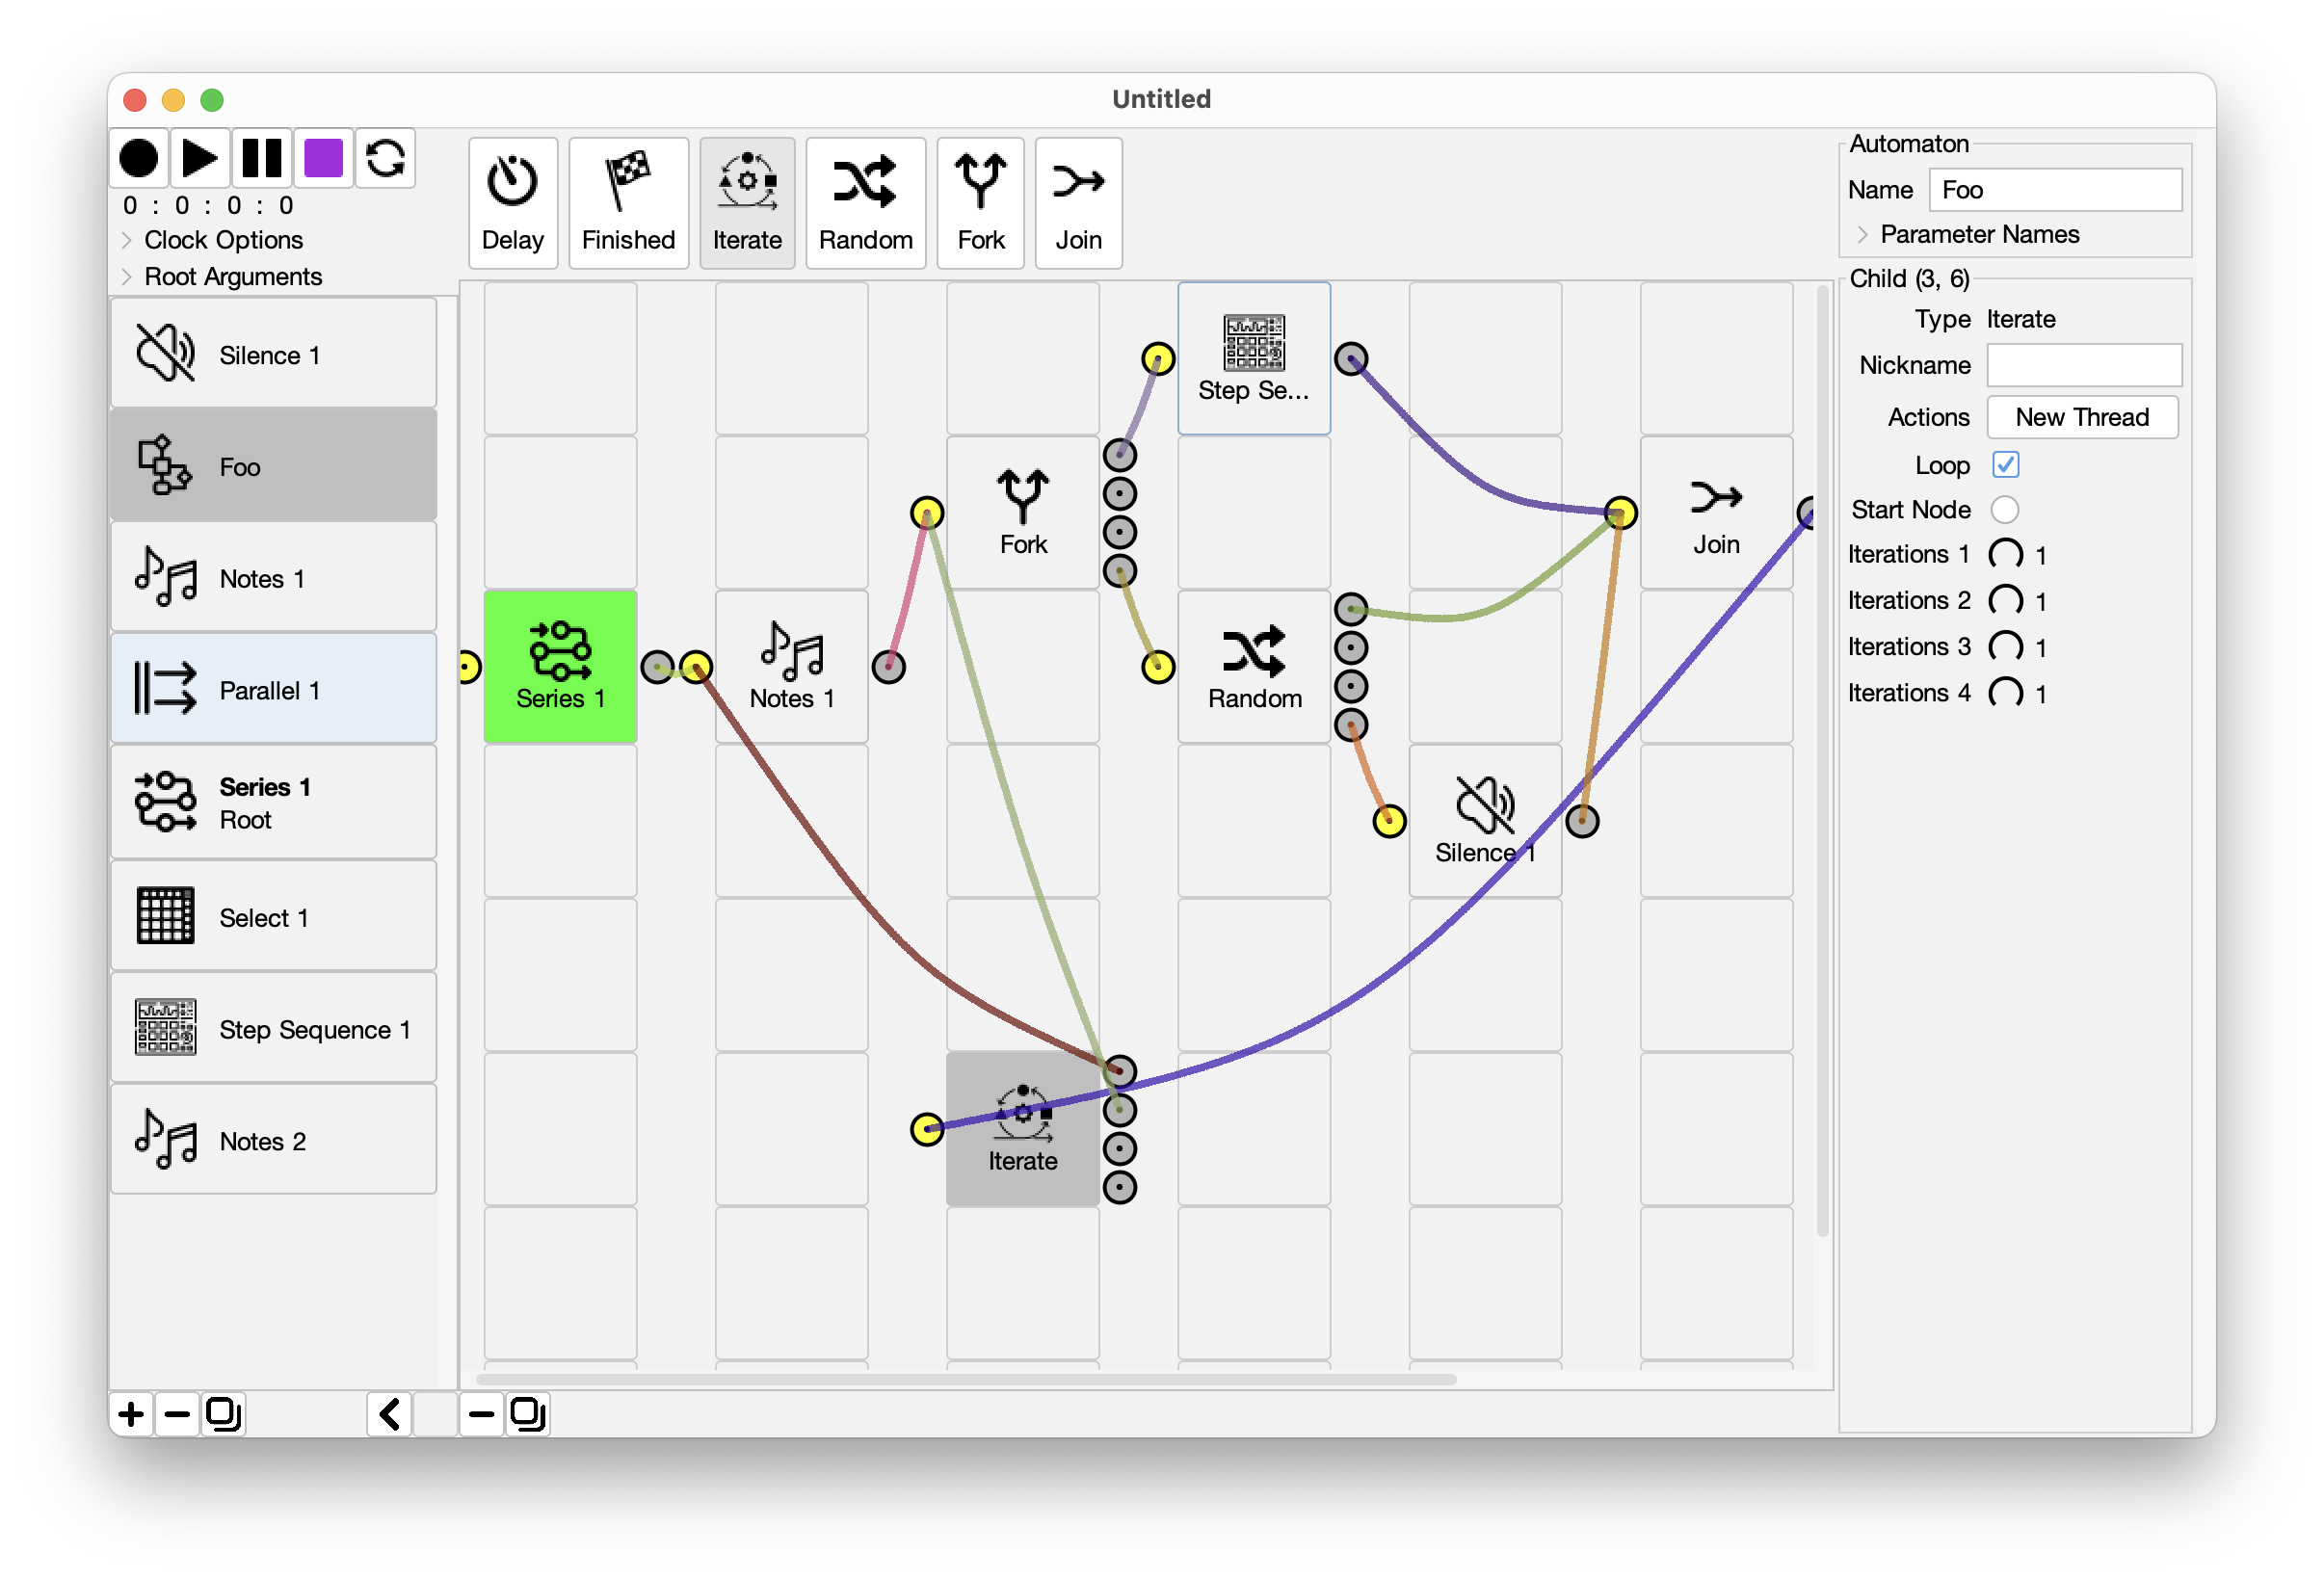
\includegraphics[width=6.5in]{Automaton}
\vspace{-2em}
\caption{Automaton Motif.}
\label{automaton}
\end{figure}

\subsection{Automaton}

Automaton may be think of as an elaborate combination of Parallel and Select.  In Automaton you lay out Children, and various decision point nodes, then connect them to construct a diagram indicating the process you want to take place.  This is known as an {\it Automaton}.  

An Automaton contains {\bf Nodes}, that is, Children and Decision Points\,---\,and {\bf Edges}, that is, connections from Node to another.  Connections go from the endpoint of a Node to the start point of a new Node.  In our Automaton, several kinds of Nodes can have multiple endpoints, but all Nodes have just one start point.  However, while can connect many Edges to the same start point, you can connect only one Edge to a given end point.

You add Children to the Automaton by dragging them in from the Motif List.  You add Decision Points to the Automaton by dragging them in from one of the six Decision Point buttons at top ({\bf Delay, Chord, Finished, Iterate, Random, Fork,} and {\bf Join}).  You can delete a Node by selecting it, then pressing the {\bf Delete Button} at bottom, and similarly you can duplicate a Node by selecting it, then pressing the {\bf Duplicate Button}.  You can move nodes to different slots by dragging them. 

Edge are connected by dragging from an endpoint to a start point.  You can delete an edge by clicking on the endpoint from which it began.

\paragraph{Playing}

The Automaton is capable of playing multiple things at one time.  The process of playing a single item is called a {\bf Thread}.   In a Thread, a single Node is playing, and when it finished playing, it passes playing on to another Node, or if it passes to nothing, the Thread is terminated.  Threads operate independently.  There can be no more than 8 Threads playing at one time.  Normally Threads are created automatically, but you can manually start a Thread on any Node by selecting the Node and clicking the {\bf Start Thread} button (if there are already 8 active threads, this button does nothing).

One Node is designated the {\bf Start Node}.  At present it's colored ugly Lime Green.  When the Automaton is started, it initiates a single Thread, playing the Start Node.  You can designate the Start Node by selecting it and then clicking on the {\bf Start Node} button in the Inspector, or selecting {\bf Make Start Node} in the {\bf Automaton} menu.

When a Node has finished playing, it will select one of its endpoints, and its Thread will start playing whatever is connected to that endpoint via an Edge.  If nothing is connected, then nothing new will play and the Thread will terminate.  If all Threads have terminated, then the Automaton itself will Finish: there's nothing left to play!

Some nodes take up time while playing: for example, a Notes object will take time to play its notes.  Indeed all Children must consume at least one Tick of time.  However many Decision Point Nodes take up zero time to play, and immediately transfer to other Nodes.  It's possible to set up a cycle (an infinite loop) of zero-time Decision Point Nodes, but Seq will detect this and force the to consume at least Tick of time.

\paragraph{Child Features}

Each Child has a {\bf Nickname} that you can set in its Inspector to make it easier to read.

While playing, a Child is played once, then played additional iterations, as designated by its {\bf Initial Repeats}.  Thereafter we flip a coin with a {\bf Repeat Probability} and each time it comes up heads, we play the Child again.  When it comes up tails, we stop playing the Child.

Alternatively if you select {\bf Until Trigger 8}, both Repeats features are ignored and the Child  will repeat forever until the Series receives a Trigger on Parameter 8.  (For discussion of Parameters, see Section~\ref{parameters}).

Each iteration of the Child stops (or restarts) at the nearest {\bf Quantization} after it has finished.  This can be {\it None} (no stop immediately), {\it 16th Note, Quarter Note,} or {\it Measure}.



\paragraph{The Decision Points}

Decision Points are not Children: when they are playing they do not cause other Motifs to play.  Instead, they are used to control the flow of the Automaton process.    Each Decision Point has a {\bf Nickname} that you can set in its Inspector to make it easier to read.  

There are six Decision Point Nodes at present:

\begin{itemize}
\item{\bf Delay}\quad While playing, this simply does nothing for a set period of time, then finishes.  You can set the amount of {\bf Delay} in Ticks, Beats, Bars (Measures), and Parts.  There are 192 Ticks per Beat, and 256 Bars per Part.  The number of Beats per Measure is set in the Clock Options.  There are {\bf Presets} in fractions of a Beat that you might find helpful.  Delay and Chord are the only Decision Points that takes up time.

\item{\bf Chord}\quad While playing, this plays a chord.  You can set the total {\bf length} in  You can set the {\bf Length} in Ticks, Beats, Bars (Measures), and Parts.  There are 192 Ticks per Beat, and 256 Bars per Part.  The number of Beats per Measure is set in the Clock Options.  There are {\bf Presets} in fractions of a Beat that you might find helpful.  Delay and Chord are the only Decision Points that takes up time.

You can also set the {\bf Gate Percentage}.  This is the percentage of the Length where the Chord actually plays.   You can specify both the {\bf Velocity} and the {\bf Release Velocity}, and of course up to four {\bf pitches} for the chord notes proper.

\item{\bf Finished}\quad This simply asks the Automaton to declare to its parent that it is Finished, and then terminates in zero time.

\item{\bf Iterate}\quad This Decision Point is used to perform elaborate controlled loops.  Iterate  has four endpoints.  When it starts playing, it terminates immediately in zero time and control continues out one the first four endpoints that is connected. When you start playing it {\it again}, it does the same thing.  This continues for the number of {\bf Iterations} designated for that endpoint.  When these iterations have been completed, it will start outputting at the {\it next} endpoint that is connected, and so on. 

If there are no more endpoints, and {\bf Loop} has been selected, then Iterations will loop back and start again with the first connected endpoint.  Otherwise it will terminate and not pass control any more.

\item{\bf Random}\quad This Decision Point is used to make random decisions.  Random has four endpoints.  When it starts playing, it terminates immediately in zero time and control continues out one of its four endpoints. The endpoint selected is done so at random using the {\bf Weights} as probabilities.  If the selected endpoint is connected, the connected Node starts playing.  Otherwise, Random terminates and does not pass control. 

\item{\bf Fork}\quad This Decision Point passes control to {\it all its endpoints at the same time}, thus allowing playing of multiple Nodes in parallel.  It does this in zero time.  New Threads are created as necessary.  If Fork cannot create enough Threads (the active thread limit of 8 would be exceeded) Threads are only created up to the maximum for the earlier endpoints, and later endpoints are ignored.

\item{\bf Join}\quad This Decision Point waits until some number \(N\) of Threads have reached its start point, and then it terminates of them, and creates a single Thread which passes control to its endpoint.  You can set \(N\) to any value from 2 to 8 (2 is the default).  Join is used to enable playing Threads to synchronize and wait for one another before terminating.  

\end{itemize}

\paragraph{MIDI Modification}
Unlike Series and Parallel, at present Automaton can exert no MIDI modification on its Children.  This might change in the future.

\clearpage

\begin{figure}[t]
\centering
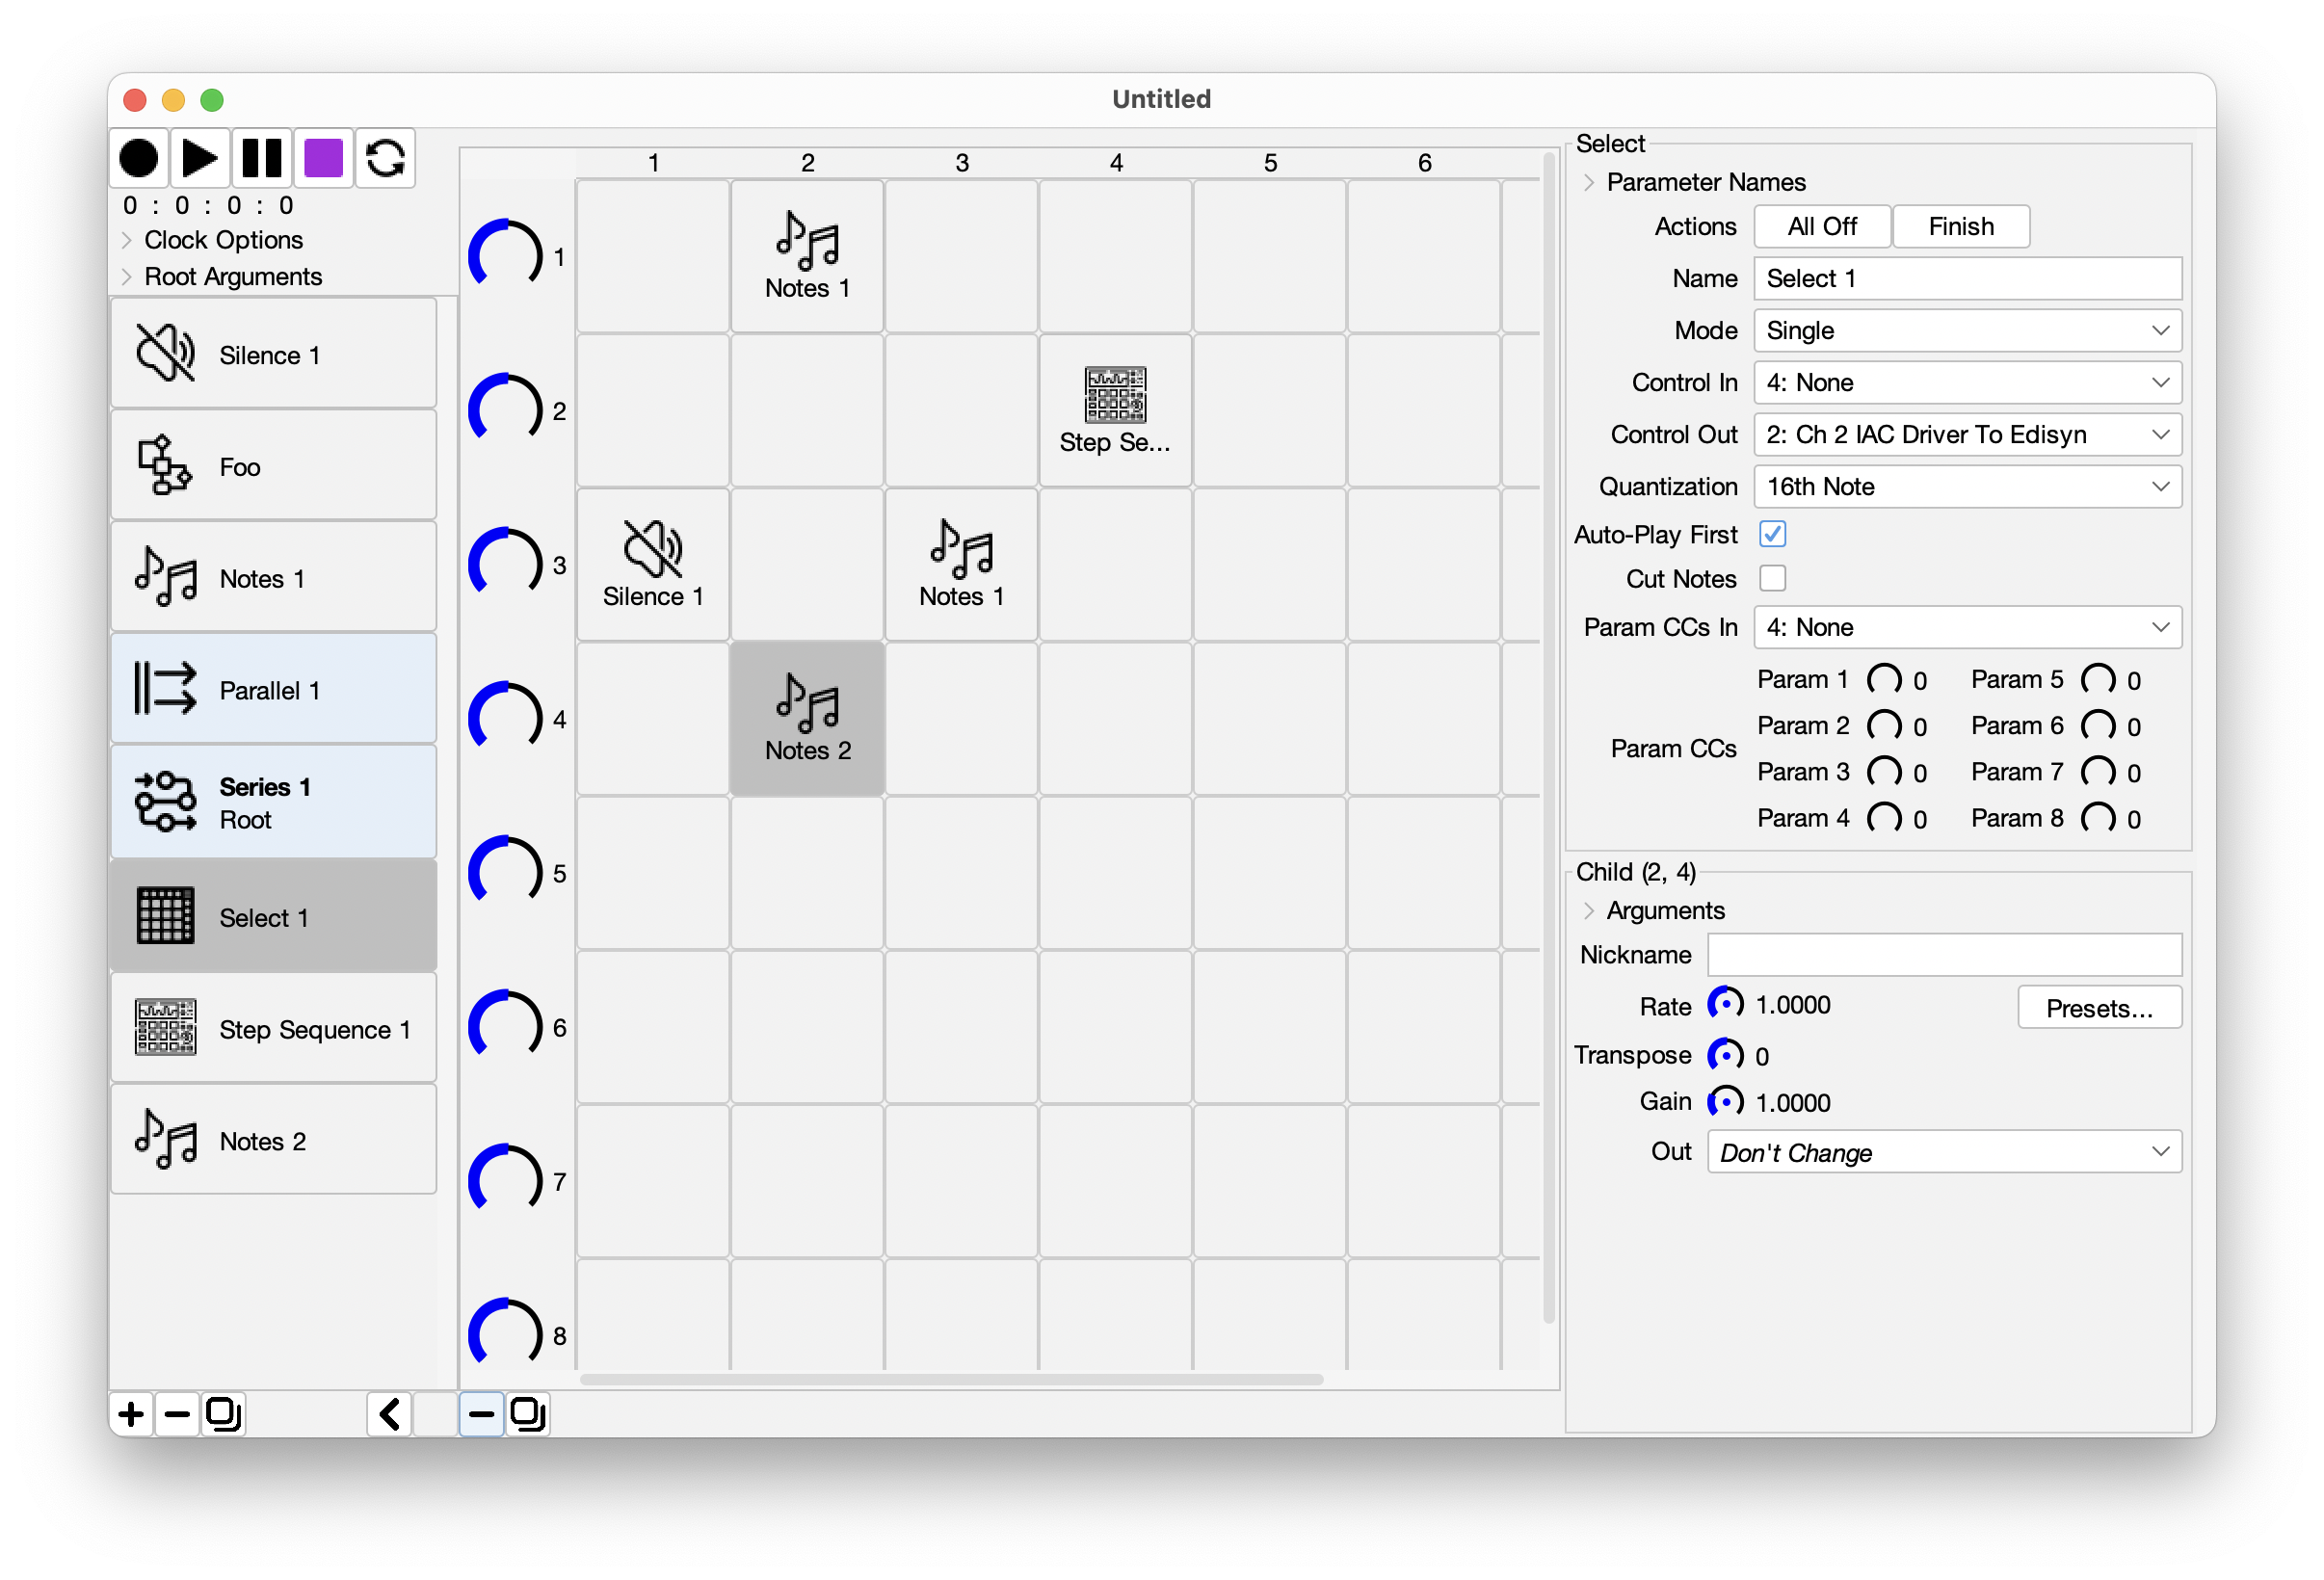
\includegraphics[width=6.5in]{Select}
\vspace{-2em}
\caption{Select Motif.}
\label{select}
\end{figure}

\subsection{Select}

Select is different from Series, Parallel, and Automaton: it has Children, but you as a user get to select which ones you want to play in real-time.  This can be done either via the user interface, or by connecting a Novation Launchpad MK III.  

Select defines a grid where you can place Children by dragging them in from the Motif List.  The location of the Children does not matter; you can lay them out however you like.  However if {\bf Auto-Play First} is selected in the Select inspector, then the first child (most top-left) will be automatically played when Select is first played.

You can drag a Child to a new location, and you can also  delete it by selecting it and pressing the {\bf Delete Button} at bottom, and similarly you can duplicate a Child by selecting it, then pressing the {\bf Duplicate Button}. 

When you click on a Child, it is selected as usual and its Inspector will come up.  But it is not chosen to start playing.  How do you do that then?  By either right-clicking on it, or holding down any modifier key (Command, Control, Shift, Option, Alt) and clicking on it.

Each Child has a {\bf Nickname} which you can set in its Inspector.  This is useful for making a shorter name for it in the grid.



Select has four modes:

\begin{itemize}
\item{\bf Single}\quad Only one Child may play at a time, but only plays once, then terminates.  If you choose a Child to play, the old Child will stop and the new one will start.  If you select a Child which is already playing, it will play again when it has finished this time.
\item{\bf Single Repeating}\quad Only one Child may play at a time, and does so over and over.  If you choose a Child to play, the old Child will stop and the new one will start.  If you select a Child which is already playing, it will stop playing.
\item{\bf Multi}\quad Multiple Children may play at a time, but each only plays once, then terminates.  If you choose a Child to play, it starts playing.   If you select a Child which is already playing, it will play again when it has finished this time.
\item{\bf Multi Repeating}\quad Multiple Children may play at a time, and each does so over and over.  If you choose a Child to play, it starts playing.  If you select a Child which is already playing, it will stop playing.
\end{itemize}

\paragraph{Quantization and Starts and Stops}

When a new Child is selected to play, and the {\bf Quantization} is set to {\it 16th Note, Quarter Note,} or {\it Measure}, then the new Child will wait until we reach the next time Quantization before it begins playing.  In the meantime, it is colored Blue.

When a new Child is selected to play, another Child may need to stop first.   If the {\bf Quantization} is set to {\it 16th Note, Quarter Note,} or {\it Measure}, then the old Child is allowed to finish playing first (and we wait until we reach the next time Quantization).  However if {\bf Quantization} is {\it None} then the old Child is terminated immediately.

Similarly, if we have terminated a Child, Quantization determines when it will stop.

\paragraph{Other Features}

At present Select has two action buttons, {\bf All Off} and {\bf Finish}.  Pressing All Off will cause Select to send an All Notes Off message to all MIDI Outs.  Pressing Finish will cause Select to tell its parent that it has Finished.  This is a rare need.

Select also can {\bf Cut Notes}.  This means that when a Child is terminated early, its notes are immediately stopped, instead of allowing the currently playing notes to finish on their own.

Select has various {\bf Param CC} options: {\color{red} these do not at present work.}  Similarly ignore the large dials to the left of the grid.

\paragraph{MIDI Modification}

As a Child of the Select emits MIDI, that MIDI is handed to the Select, which has a chance to modify it before it is passed on.  There are several available features for modification of a given Child's MIDI in its Inspector.  {\bf Transpose} transposes all notes by some number of semitones up or down.  {\bf Restrict} forces the notes to line up with notes in a given scale: notes that don't match are transposed down to the nearest note in the scale.  {\bf Gain} changes the overall volume (velocity) of notes.  And {\bf Out} changes the MIDI Out being used (by default it is set to {\it Don't Change}.

Finally, {\bf Rate} changes the speed at which the child is played, faster or slower.  Keep in mind that Seq has a resolution of 192 ticks per beat (PPQ), so changing the speed\,---\,particularly faster\,---\,can quickly result in inaccuracies.    Some {\bf Presets} are provided, including a Custom Rate option)


\paragraph{Parameters and Arguments}

The Parallel Inspector has an expandable region called {\bf Parameter Names}, and each Child Inspector has an expandable region called {\bf Arguments}. Furthermore, many dials have Special Values called ``Rand'', ``Param 1'', etc.  These are explained in Section~\ref{parameters}.


\paragraph{Using the Novation LaunchPad}

To use a Novation LaunchPad to select Children, you specify it in the {\bf Control In} and {\bf Control Out}.  You should use the Novation LaunchPad's {\bf MIDI IN} and {\bf MIDI OUT} devices, not its {\bf DAW IN} nor {\bf DAW OUT} ones.  When the Select starts playing, it will reset the Launch Pad to display the same grid as your current user interface layout.  You can then choose Children by pressing buttons on the LaunchPad.



\clearpage\subsection{Motifs Planned for the Future}

At present we have four motifs planned:

\begin{itemize}
\item A Motif for individual notes, chords, or arpeggios
\item A Motif which implements functions that operates on Parameters, such as LFOs or Envelopes, Random Sequences, MIDI CC
\item Possibly a Motif which performs more complex MIDI Effects on incoming MIDI data
\item Possibly a Motif which does Live Coding using some programming language
\end{itemize}

\clearpage

\begin{figure}[t]
\centering
\includegraphics[width=6.5in]{Macro}
\vspace{-2em}
\caption{A Macro with Two Macro Children.}
\label{macro}
\end{figure}

\section{Macros and Macro Children}

A {\bf Macro} is a whole Seq sequence DAG bundled up into a single Motif.  When the Motif is played, the underlying sequence is played until it is finished.

To create a basic Macro, you first save our your sequence.  (Remember that the sequence is saved out starting at the Motif Root, ignoring its parents and other non-descendant Motifs.)  Then you add a Macro to the Motif List and when you do it will prompt you to load that sequence into the Macro.    When you play the Macro, its stored sequence is played as-is.

This has some usefulness, but Macro can go further than this.  You can add special Motifs to your sequence called {\bf Macro Children}.  A Macro Child has a single Inspector feature: its {\bf Name}: come up with a good name for it.  If you have Macro Children in the sequence you have saved out, they become temporary placeholders for actual Children of the Macro in  your main sequence.

This means that if you had three Macro Children nodes in your macro's internal sequence for example, then the Macro itself will take up to three Children.  As the Macro is playing, it will reach its Macro Children nodes, and instead of playing them, the Macro will play the corresponding Child attached to it.  Figure~\ref{macro} shows a Macro loaded that had two Macro Children nodes inside, and thus has two slots for Children, which we have populated with a Notes and a Series from the Macro List respectively.

What's the point of this?  It allows you to use Macros to create patterns or templates, and then populate the templates with different Children as you see fit later on. 

The Child slots of a Macro are populated in the usual way: by dragging from the Motif List.  You can also clear a slot by pressing the {\bf Delete Button} below, or duplicate a Child to the next slot by selecting it and pressing the {\bf Duplicate Button}.  You can change the Name of the underlying Macro Child node: this is now the {\bf nickname} of the Child in its Inspector.

\clearpage\section{Parameterization}
\label{parameters}

\paragraph{\color{red} Warning}  Parameterization is a work in progress.  It works, but there are a lot of wires sticking out, and its value at present is limited.  Only certain Motifs support Parameterization because we started on them and haven't gotten to the others yet.

\vspace{1em}

\begin{wrapfigure}{r}{1.25in}
\vspace{-1em}
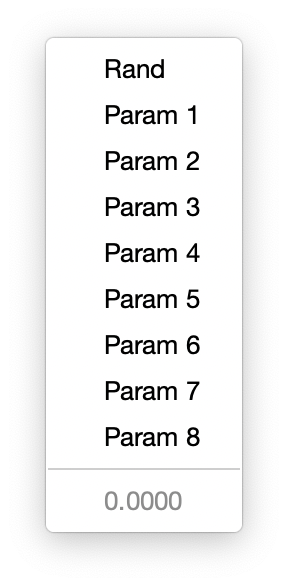
\includegraphics[width=1.25in]{params}
\vspace{-2em}
\caption{Parameters as Special Variables}
\label{params}
\end{wrapfigure}

When a Motif is played, you can also set up to eight numerical {\bf Parameters} to values to control it.  This ultimately will allow you to do things like change the Swing or the rate several Motifs together; or to automatically change the volume of a Mofif using an LFO, for example.  It's a lot like passing parameters into functions when you make function calls in a programming language.  Parameterization is complex and counterintuitive, but we'll do our best here.

A Motif has eight parameters, by default named {\bf Param 1 ... Param 8}.  You can change the names of these parameters in the {\bf Parameter Names} expandable section of the Motif's Inspector.  The Motif also has a special parameter called {\bf Rand} which provides a random number.

Many Motifs have numerical features with {\bf special values} that allow them to be bound to the value of one of the Motif's Parameters.  For example, some feature (Swing?  Gain?) of the Step Sequence's Child Inspectors might have the special variables shown at right in Figure~\ref{params}.  What are these?  These allow the musician to not just set feature to a number, but to set them to {\it whatever the Step Sequence's Parameter 4 is currently set to} for example).  If the musician changes Parameter 4, then the feature will be changed as well.

Now, Parameters are real-valued numbers from 0.0 to 1.0, but perhaps the feature is not; it might be integers, say.  If you set Parameter 4 to 0.2314, how what value is that in the feature?  It's spread over the range of values for the feature.  But one thing that can help you is the grayed-out number on the bottom of the figure at right.  That's the numerical parameter value that would correspond to the current feature value.  

\paragraph{Triggers} The Series and Automaton motifs have special options to repeat children forever until receiving a {\bf trigger} on Parameter 8.  What is a trigger?  It's just Parameter 8 going from a value less than 0.5 to a value greater to or equal to 0.5.  

\begin{wrapfigure}{r}{2.25in}
\vspace{-1em}
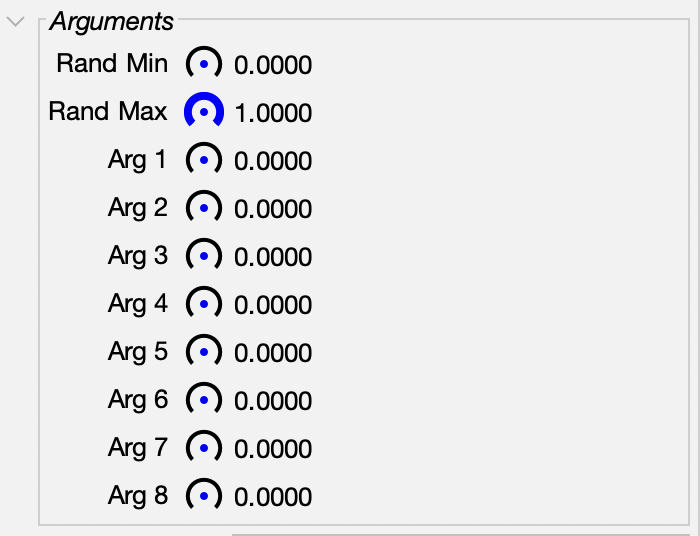
\includegraphics[width=2.25in]{arguments}
%\vspace{-2em}
\caption{Arguments with default settings.}
\label{arguments}
\end{wrapfigure}

\paragraph{Arguments}

In a Child Inspector, you can often set the {\bf arguments} of the Child.  These are the values which are passed into the Child's parameters by its parent when the Child is played.    You can set them to fixed values (like 0.2314), which will in turn change any of the Child's features that have been bound to those particular parameters.

But arguments can also {\it themselves be bound} to the parent's parameters.  For example, you could bind Argument 4 of a child of a Series to Parameter 5 of the Series itself.  This means that when the musician changes Parameter 5 of the Series, then Argument 4 of the Child is also changed, and thus the feature of the Child is changed as well!  Thus parameter values can be passed down from parent to child to grandchild etc.

\paragraph{A Warning about Child Arguments}

Consider the Series motif. Each of its children can have (for example) Fixed Repeats.  These can be bound to parameters.  But note that these features are not features of the Child: they are features of the Series, and thus they are bound to the Series's parameters, not to the Child parameters, and thus you don't set them with the Childs's arguments.

This can be a little confusing.  In short, if a feature appears anywhere in {\it any Inspector} associated with a Motif (the Motif Inspector, one of its Child inspectors, etc.), that feature {\it belongs to the Motif} when it comes to parameterization.  

\begin{wrapfigure}{r}{1.25in}
\vspace{-1em}
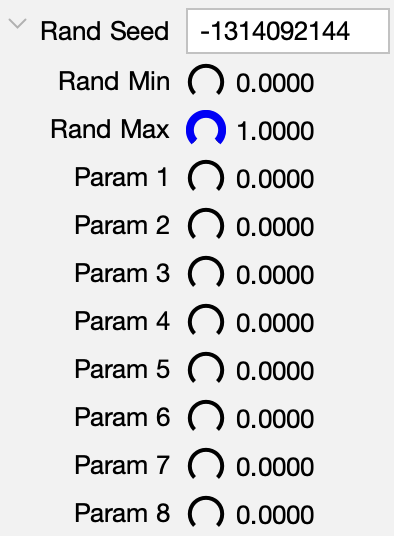
\includegraphics[width=1.25in]{rootarguments}
%\vspace{-2em}
\caption{Root Arguments with default settings.}
\label{rootarguments}
\end{wrapfigure}

\paragraph{The Root Arguments}  If the Root Motif has bound things to its parameters, where are those arguments set?  They're set in the Root Arguments, located below the Transport.

\paragraph{Parameter Updates}  Parameters are updated every single Tick (192 times per beat).

\paragraph{The Random Parameter}  In addition to eight parameters, you can also bind a feature to the {\bf Random Parameter} (or {\bf Rand}).  This parameter is always set to a random value.  The value is not changed as often as other arguments: it is changed only each time the motif starts playing.

The Random Parameter is set to a random value between the {\bf Random Min} and {\bf Random Max} inclusive.  You can set these as arguments in the parent (and yes, you can bind them).  

\paragraph{The Point}  Parameterization is very powerful for automation and global control of many features at once, but we're not sure just how many features will benefit from parameterization and how useful it will be.    Time will tell.

\end{document}





